\section{Celda Rauch (Deliyannis - Friend modificada)}
En esta secci\'on se detalla el proceso de dise\~no e implementaci\'on de un filtro pasabanda que cumple con las caracter\'isticas detalladas en la Tabla \ref{tab:FILTER_SPECS}. Se utiliza para encontrar una transferencia que cumpla con la plantilla, la aproximaci\'on de Chebyshev, y para la implementaci\'on del circuito, la celda Rauch de baja se\~nal.
\begin{table}[H]
    \centering
    \resizebox{0.5\textwidth}{!}{%
    \begin{tabular}{cc}
    \hline
    \multicolumn{2}{c}{Par\'ametros de diseño} \\ \hline
    Pendiente de pasabajos normalizado & -40dB/dec \\
    $f_p$ & 36KHz \\
    B & 1/10 \\
    $A_p$ & 3dB \\
    $|Z_{in}(f)|$ & $\geq 50K\Omega$ \\
    Filtro & Pasa-Banda\\\hline
    \end{tabular}%
    }

    \caption{Par\'ametros de diseño para el filtro a implementar}
    \label{tab:FILTER_SPECS}
    \end{table}
\subsection{Celda a utilizar y justificaci\'on}
Se presenta en la Figura \ref{fig:RAUCH_SIMPLE} la celda pasabanda Rauch simple, que es la ultilizada generalmente en el dise\~no de filtros con dicha celda. 
\begin{figure}[H]
    \centering
    \resizebox{0.7\textwidth}{!}{% 
        \includegraphics[scale=0.4]{../EJ2/Recursos/RAUCH_SIMPLE}
    }
    \caption{Celda Rauch simple}
    \label{fig:RAUCH_SIMPLE}
\end{figure}
Sin embargo, se observa que uno de los requisitos que debe cumplir el filtro es que $B = \frac{1}{Q} = 10$. Este valor de Q hace que,  las relaciones entre las resistencias R1 y R2 sea muy dispar, puesto que los valores de estas resistencias son inversa y directamente proporcionales, respectivamente, a este valor.

En base a lo tratado en la bibliograf\'a utilizada \footnote{\label{fn:SCHAUMANN}Rolf Schaumann, Mac van Valkenburg, Design of analog filters (Oxford University Press 2001)} se decide utilizar la versi\'on mejorada de esta celda. Las resistencias conservar la misma relaci\'on con el factor de calidad del circuito.La diferencia se encuentra en que se hace mas peque\~no este valor, pero aplicando una peque\~na realimentaci\'on positiva al amplificador operacional se logra mantener el factor de calidad deseado cambiando los valores de las resistencias en dicha realimentaci\'on. Es de suma importancia remarcar que, al agregar estas resistencias en la realimentaci\'on, se reduce considerablemente el error debido al $A_{vol}$ del ampificador, en la frecuencia de corte y en el factor de calidad. Se hace un an\'alisis con mayor profundidad de esta caracter\'istica en las siguiente secciones.

Se presenta en la Figura \ref{fig:ENHANCED_RAUCH} el circuito que se propone y el que se utiliza en las siguientes secciones para realizar el an\'alisis. Es
\begin{figure}[H]
    \centering
    \resizebox{0.7\textwidth}{!}{%        
        \includegraphics{../EJ2/Recursos/ENHANCED_RAUCH}       
    }
    \caption{Celda Rauch mejorada}
    \label{fig:ENHANCED_RAUCH}
\end{figure}


\subsection{Celda Rauch pasabanda: An\'alsis ideal}
\label{sec:IDEAL_ANALISIS}
En esta secci\'on se considera al amplificador de la celda como ideal, es decir impedancia de entrada $Z_{IN}$ infinita, impedancia de salida $Z_{OUT}$ nula, y $A_{vol}$ infinito e invariante con la frecuencia.

Este an\'alisis permite obtener una primera aproximaci\'on al funcionamiento de la celda con una precisi\'on correcta. Adem\'as de la transferencia ideal, se analiza  a continuaci\'on  las caracter\'isticas de dise\`no propuestas, las sensibilidades, la impedancia de entrada y salida del sistema y finalmente el rango din\'amico.   
\subsubsection{Tranferencia y caracter\'isticas}
Se parte del sistema de ecuaciones  \ref{eq:SIST_GEN} 
\begin{equation}
    \left\{
        \begin{array}{lll}
            {\it VA}={\frac {{\it Vout}\,{\it RA}}{{\it RB}+{\it RA}}}\\
            \left( {\it Vx}-{\it VA} \right) s{\it C2}+{\frac {{\it Vx}}{{\it R2}
            }}+ \left( {\it Vx}-{\it Vout} \right) s{\it C1}={\frac {{\it Vin}-{
            \it Vx}}{{\it R1}}}\\
            \left( {\it Vx}-{\it VA} \right) s{\it C2}= \left( {\it VA}-{\it Vout
            } \right) {\it R3}

        \end{array}
    \right.
    \label{eq:SIST_GEN}
\end{equation}

Se obtienen entonces las caracter\'isticas del sistema mostradas en \ref{eq:SOLUC_GEN}
\begin{equation}    
    \centering
        \begin{split}  
            &H(s) = -{\frac {{\it C2}\,{\it R2}\,s \left( {\it RB}+{\it RA} \right) }{{
                \it C1}\,{\it C2}\,{\it R1}\,{\it R2}\,{\it RB}\,{s}^{2}+ \left( {\it 
                C1}\,{\it R1}\,{\it R2}\,{\it R3}\,{\it RB}+{\it C2}\,{\it R1}\,{\it 
                R2}\,{\it R3}\,{\it RB}-{\it C2}\,{\it R1}\,{\it RA}-{\it C2}\,{\it R2
                }\,{\it RA} \right) s+{\it R1}\,{\it R3}\,{\it RB}+{\it R2}\,{\it R3}
                \,{\it RB}}}\\
            &{{\it \omega_0}}^{2}={\frac {{\it R3}\, \left( {\it R1}+{\it R2} \right) }{{
                    \it C1}\,{\it C2}\,{\it R1}\,{\it R2}}}\\
            &Q={\frac {{\it C1}\,{\it C2}\,{\it R1}\,{\it R2}\,{\it RB}\,{\it 
            \omega_0} }{{\it C1}\,{\it R1}\,{
                \it R2}\,{\it R3}\,{\it RB}+{\it C2}\,{\it R1}\,{\it R2}\,{\it R3}\,{
                \it RB}-{\it C2}\,{\it R1}\,{\it RA}-{\it C2}\,{\it R2}\,{\it RA}}} \\
        \end{split}    
    \label{eq:SOLUC_GEN}
\end{equation}


\subsubsection{Caracter\'isticas de dise\~no}
Al dise\~nar un filtro de varias etapas se distribuyen polos y ceros de la transferencia deseada entre dichas etapas. Para esto existen algunos m\'etodos de elecci\'on de valores que cumplan con los requerimientos y que se obtenga una mejor sensibilidad en los componentes. Un ejemplo es el dise\~no por componentes iguales o el dise\~no por componentes proporcionales, ambos tratados en profundidad en el punto anterior. 

Sin embargo, y siguiendo con el dise\~no propuesto en la bibliograf\'ia$^{\ref{fn:SCHAUMANN}}$, se propone una mezcla de ambos m\'etodos. Se muestra en la Figura \ref{fig:RAUCH_VALUES}
\begin{figure}[H]
    \centering
    \resizebox{0.7\textwidth}{!}{% 
        \includegraphics[scale=0.5]{../EJ2/Recursos/RAUCH_VALUES}
    }
    \caption{Criterio de dise\~no propuesto}
    \label{fig:RAUCH_VALUES}
\end{figure}
Al utilizar esta estrategia se logran minimizar las sensibilidades de $\omega_0$ y Q. Adem\'as aparecen par\'ametros que relacionan a componentes, lo que facilita la selecci\'on de valores para los mismos, ya que al fijar el valor para uno de ellos, el resto se obtienen a partir de la relaci\'on. 
Es posible entonces expresar tanto la transferencia de la celda como $\omega_0 $ y Q como se muestra en \ref{eq:SOLUC_NEW_DESIGN}

\begin{equation}    
        \begin{split}    
            &H(s) = -\frac{1}{1-K}\cdot \frac{\frac{a\cdot s}{R1\cdot C}}{s^2+\frac{2}{R2\cdot C}\cdot \left(1+\frac{K}{K-1}\cdot \frac{R2}{2\cdot R1}\right)\cdot s+\frac{1}{C^2\cdot R1 \cdot R2}}\\
            &{{\it \omega_0}}^2=\frac{1}{C^2\cdot R1 \cdot R2}\\
            &Q=\frac{R2\cdot C\cdot \omega_0}{2\cdot\left(1+\frac{K}{K-1}\cdot \frac{R2}{2\cdot R1}\right)}\\
           & H_P = -\frac{1}{1-K}\cdot \frac{\frac{a\cdot }{R1\cdot C}}{\frac{2}{R2\cdot C}\cdot \left(1+\frac{K}{K-1}\cdot \frac{R2}{2\cdot R1}\right)}
        \end{split}    
    \label{eq:SOLUC_NEW_DESIGN}
\end{equation}
Se puede observar que, debido a la menor cantidad de variables y longitud de las expresiones obtenidas, es posible extraer conclusiones a partir de ellas de una manera m\'as sencilla.

\subsubsection{Impedancia de entrada}
Se presenta a continuaci\'on el c\'alculo de impedancia de entrada bajo la suposici\'on de  idealidad.

Cabe recalcar que el c\'alculo de la impedancia de entrada y de salida es de suma importancia para el dise\~no de filtros compuestos por varias etapas. Esto es debido a que al conectarlos en cascada, se espera que la transferencia del sistema sea el producto de las etapas que lo componen. Para lograrlo, es necesario que la impedancia de salida de una etapa sea mucho menor que la impedancia de entrada de la etapa siguiente. Se logra entonces, que las etapas no se carguen mutuamente y que las transferencias no se vean afectadas.

Se parte del sistema de ecuaciones \ref{eq:SIST_ZIN}.
\begin{equation}    
    \left\{
        \begin{array}{ll}
            Z_{IN} = \frac{V_{IN}}{I_{IN}}\\
            I_{IN} = \frac{V_{IN}-V_X}{\frac{R1}{a}}
            
        \end{array}
    \right.
    \label{eq:SIST_ZIN}
\end{equation}
Se puede observar en \ref{eq:ZIN} la expresi\'on obtenida para la impedancia de entrada. 

\begin{equation}
    Z_{IN}(s) =R1\cdot \frac{ C^2 R1 R2\cdot (K-1) \cdot s^2 + 2 C R1\left( K+\frac{K R2}{2 R1} - 1\right) \cdot s + (K+1)  }{C^2 R1 R2\cdot (K-1) \cdot s^2+2 C R1\left( \frac{R2}{2 R1} \cdot K \cdot(1-a) +(1-a) + (K-1)\right) \cdot s + K\cdot (1-a)+ a -1}
    \label{eq:ZIN}
\end{equation}

A partir de la expresi\'on de la impedancia de entrada es posible observar la dependencia directa del valor de la impedancia de entrada, con el valor elegido para el pa\'ametro R1. Es de suma importancia realizar correctamente la elecci\'on de este valor para garantizar que la impedancia de entrada de las etapas sea lo m\'as alta posible y as\'i asegurar un correcto desacople entre estas.

Si bien se realiz\'o un an\'alisis para encontrar los m\'inimos de la impedancia de entrada para obtener un par\'ametro adicional al momento de realizar la selecci\'on de los componentes, las expresiones gen\'ericas no permiten extraer conclusiones debido a su complejidad. Se decide por lo tanto no incluirlo en este trabajo. 


\subsubsection{Impedancia de salida}
En el caso del an\'alisis ideal el c\'alculo de la impedancia de salida es trivial. Al ser la salida del sistema, la salida de un amplificador operacional con realimentaci\'on negativa, la haber una variac\'ion en la salida, el sistema evoluciona para manterner la salida constante. Por lo tanto, se obtiene la conclusi\'on de que en el caso ideal la impedancia de salida debe ser necesariamente 0.

\subsubsection{Sensibilidades}
En el siguiente an\'alisis se emplea la definici\'on de sensibilidades relativas para cada una de las magnitudes o par\'ametros caracter\'isticos de la funci\'on transferencia. Esto es,
calcular $S^{y}_x = \frac{x_o}{y(x_o)} \cdot \frac{\delta y}{\delta x}$.
Si bien se define el circuito con par\'ametros relacionales que facilitan su dise\~no, es importante calcular las sensibilidades respecto a todos los componentes del circuito. En el caso se K, se mantiene en el circuito pues los valores de las resistencias no aportan informaci\'on relevante al comportamiento del circuito, sino que solamente es de inter\'es la relaci\'on entre ellas, y en base a eso se hace el estudio de sensibilidades.
Se presenta en la Figura \ref{fig: CIRC_SENS} el circuito utilizado para relizar el c\'alculo de las sensibilidades. La expresiones de las que se parte para realizar los c\'alculos no se agregan al informe pues no aportan informac\'on adicional ya que coinciden con las halladas anteriormente, simplemente que con un grado de complejidad menor. En pocas palabras, es posible utilizar convenientemente las ecuaciones halladas anteriormente.\begin{figure}[H]
    \centering
    \resizebox{0.7\textwidth}{!}{%        
        \includegraphics{../EJ2/Recursos/CIRC_SENS}       
    }
    \caption{Celda Rauch utilizada para el c\'alculo de sensibilidades}
    \label{fig: CIRC_SENS}
\end{figure} 
Se muestran en las Tablas \ref{tab:SENS_W_HP} y \ref{tab:SENS_Q} las sensibilidades obtenidas.
\begin{table}[H]
\centering
\begin{tabular}{ccc}
\hline
Componente & $S_X^{\omega_0}$ & $S_X^{H_P}$ \\ \cline{1-3}\\
$R_1$  & $-{\frac {{\it R3}}{ 2.0\,{\it R1}+ 2.0\,{\it R3}}}$    &$ -{\frac { \left( {\it C1}\,K{\it R3}+K{\it R2}\,{\it C2}+{\it C2}\,K{
\it R3}-{\it C1}\,{\it R3}-{\it C2}\,{\it R3} \right) {\it R1}}{{\it 
C1}\,K{\it R1}\,{\it R3}+K{\it R2}\,{\it C2}\,{\it R1}+{\it C2}\,K{
\it R1}\,{\it R3}+K{\it R2}\,{\it C2}\,{\it R3}-{\it C1}\,{\it R1}\,{
\it R3}-{\it C2}\,{\it R1}\,{\it R3}}} $  \\
$R_2$  & -0.5    & ${\frac {{\it R1}\,{\it R3}\, \left( {\it C1}\,K+{\it C2}\,K-{\it C1}-{
\it C2} \right) }{{\it C1}\,K{\it R1}\,{\it R3}+K{\it R2}\,{\it C2}\,{
\it R1}+{\it C2}\,K{\it R1}\,{\it R3}+K{\it R2}\,{\it C2}\,{\it R3}-{
\it C1}\,{\it R1}\,{\it R3}-{\it C2}\,{\it R1}\,{\it R3}}}$   \\
$R_3$  & $-{\frac {{\it R1}}{ 2.0\,{\it R1}+ 2.0\,{\it R3}}}$     & ${\frac {K{\it R2}\,{\it C2}\,{\it R1}}{{\it C1}\,K{\it R1}\,{\it R3}+K
{\it R2}\,{\it C2}\,{\it R1}+{\it C2}\,K{\it R1}\,{\it R3}+K{\it R2}\,
{\it C2}\,{\it R3}-{\it C1}\,{\it R1}\,{\it R3}-{\it C2}\,{\it R1}\,{
\it R3}}}$   \\
$C_1$  & -0.5    & $-{\frac { \left( K{\it R2}\,{\it R1}+{\it R1}\,{\it R3}\,K+K{\it R2}\,
{\it R3}-{\it R1}\,{\it R3} \right) {\it C2}}{{\it C1}\,K{\it R1}\,{
\it R3}+K{\it R2}\,{\it C2}\,{\it R1}+{\it C2}\,K{\it R1}\,{\it R3}+K{
\it R2}\,{\it C2}\,{\it R3}-{\it C1}\,{\it R1}\,{\it R3}-{\it C2}\,{
\it R1}\,{\it R3}}}$ \\  

$C_2$  & -0.5    & $-{\frac {{\it R3}\,{\it R1}\, \left( -1+K \right) {\it C1}}{{\it C1}\,
K{\it R1}\,{\it R3}+K{\it R2}\,{\it C2}\,{\it R1}+{\it C2}\,K{\it R1}
\,{\it R3}+K{\it R2}\,{\it C2}\,{\it R3}-{\it C1}\,{\it R1}\,{\it R3}-
{\it C2}\,{\it R1}\,{\it R3}}}$  \\
 $K$ & 0&$-\frac{2KR_1R_2+KR_3(R_1+R_2)}{2R_1R_2(K-1)+KR_3(R_1+R_2)}$  \\
\hline
\end{tabular}
\caption{Tabla de sensibilidades de $\omega_0$ y de la ganancia en la banda pasante}
\label{tab:SENS_W_HP}
\end{table}
\begin{table}[H]
\centering
\begin{tabular}{cc}
\hline
Componente & $S_X^{Q}$ \\ \hline\\
$R_1$  & $1/2\,{\frac {{\it R3}\, \left( K{\it R2}\,{\it C1}\,{\it R1}-{\it C1}
\,K{\it R1}\,{\it R3}+K{\it R2}\,{\it C1}\,{\it R3}-{\it C2}\,K{\it R1
}\,{\it R3}+{\it C1}\,{\it R1}\,{\it R3}+{\it C2}\,{\it R1}\,{\it R3}
 \right) }{ \left( K{\it R2}\,{\it C1}\,{\it R1}+{\it C1}\,K{\it R1}\,
{\it R3}+K{\it R2}\,{\it C1}\,{\it R3}+{\it C2}\,K{\it R1}\,{\it R3}-{
\it C1}\,{\it R1}\,{\it R3}-{\it C2}\,{\it R1}\,{\it R3} \right) 
 \left( {\it R1}+{\it R3} \right) }}$ \\
$R_2$  & $-1/2\,{\frac {K{\it R2}\,{\it C1}\,{\it R1}-{\it C1}\,K{\it R1}\,{\it 
R3}+K{\it R2}\,{\it C1}\,{\it R3}-{\it C2}\,K{\it R1}\,{\it R3}+{\it 
C1}\,{\it R1}\,{\it R3}+{\it C2}\,{\it R1}\,{\it R3}}{K{\it R2}\,{\it 
C1}\,{\it R1}+{\it C1}\,K{\it R1}\,{\it R3}+K{\it R2}\,{\it C1}\,{\it 
R3}+{\it C2}\,K{\it R1}\,{\it R3}-{\it C1}\,{\it R1}\,{\it R3}-{\it C2
}\,{\it R1}\,{\it R3}}}$ \\
$R_3$  & $1/2\,{\frac {{\it R1}\, \left( K{\it R2}\,{\it C1}\,{\it R1}-{\it C1}
\,K{\it R1}\,{\it R3}+K{\it R2}\,{\it C1}\,{\it R3}-{\it C2}\,K{\it R1
}\,{\it R3}+{\it C1}\,{\it R1}\,{\it R3}+{\it C2}\,{\it R1}\,{\it R3}
 \right) }{ \left( K{\it R2}\,{\it C1}\,{\it R1}+{\it C1}\,K{\it R1}\,
{\it R3}+K{\it R2}\,{\it C1}\,{\it R3}+{\it C2}\,K{\it R1}\,{\it R3}-{
\it C1}\,{\it R1}\,{\it R3}-{\it C2}\,{\it R1}\,{\it R3} \right) 
 \left( {\it R1}+{\it R3} \right) }}$ \\
 $C_1$  & $1/2\,{\frac {K{\it R2}\,{\it C1}\,{\it R1}+{\it C1}\,K{\it R1}\,{\it 
R3}+K{\it R2}\,{\it C1}\,{\it R3}-{\it C2}\,K{\it R1}\,{\it R3}-{\it 
C1}\,{\it R1}\,{\it R3}+{\it C2}\,{\it R1}\,{\it R3}}{K{\it R2}\,{\it 
C1}\,{\it R1}+{\it C1}\,K{\it R1}\,{\it R3}+K{\it R2}\,{\it C1}\,{\it 
R3}+{\it C2}\,K{\it R1}\,{\it R3}-{\it C1}\,{\it R1}\,{\it R3}-{\it C2
}\,{\it R1}\,{\it R3}}}$ \\
$C_2$  & $-1/2\,{\frac {K{\it R2}\,{\it C1}\,{\it R1}+{\it C1}\,K{\it R1}\,{\it 
R3}+K{\it R2}\,{\it C1}\,{\it R3}-{\it C2}\,K{\it R1}\,{\it R3}-{\it 
C1}\,{\it R1}\,{\it R3}+{\it C2}\,{\it R1}\,{\it R3}}{K{\it R2}\,{\it 
C1}\,{\it R1}+{\it C1}\,K{\it R1}\,{\it R3}+K{\it R2}\,{\it C1}\,{\it 
R3}+{\it C2}\,K{\it R1}\,{\it R3}-{\it C1}\,{\it R1}\,{\it R3}-{\it C2
}\,{\it R1}\,{\it R3}}}$ \\
$K$  &$\frac{KR_3(R_1+R_2)}{(K-1)(R_1((K-1)2R_2+KR_3)+KR_2R_3)}$ \\    
\hline
\end{tabular}
\caption{Tabla de sensibilidades de Q}
\label{tab:SENS_Q}
\end{table}

\subsection{Celda Rauch pasabanda: An\'alsis real}
En esta secci\'on se repite el an\'alisis realizado anteriormente pero sin la consideracion de $A_{vol}$ infinito e invariante con la frecuencia. En este caso, se considera $A_{vol}$ finito y, adem\'as, su respectiva variaci\'on con la frecuencia en concordancia con el polo dominante.


\subsubsection{Tranferencia y caracter\'isticas}
En este caso, para hallar la transferencia, se parte del sistema de ecuaciones \ref{eq:SIST_REAL}.
\begin{equation}
    \left\{
        \begin{array}{lll}
            {\it VA}={\frac {{\it Vout}\,{\it RA}}{{\it RB}+{\it RA}}}\\
            \left( {\it Vx}-{\it VA} \right) s{\it C2}+{\frac {{\it Vx}}{{\it R2}
            }}+ \left( {\it Vx}-{\it Vout} \right) s{\it C1}={\frac {{\it Vin}-{
            \it Vx}}{{\it R1}}}\\
            \left( {\it Vx}-{\it VA} \right) s{\it C2}= \left( {\it VA}-{\it Vout
            } \right) {\it R3}

        \end{array}
    \right.
    \label{eq:SIST_REAL}
\end{equation}
De este sistema, y luego de operar sobre el resultado obtenido, se llega a la expresi\'on de la transferencia mostrada en \ref{eq:TRANS_REAL}.
\begin{equation}
    \begin{split}
        &H(s) = \frac{s\cdot a}{C R1 \alpha} \cdot \frac{1}{s^2+\frac{2}{C R2 \alpha}\cdot \left(\alpha + \frac{R2(A_{vol}-1)}{2 A_{vol} R1} \right)\cdot s +\frac{1}{C^2 R1 R2}}\\
        &{{\it \omega_0}}^2=\frac{1}{C^2\cdot R1 \cdot R2}\\
        &Q = \frac{ \omega_0}{\frac{2}{C R2 \alpha}\cdot \left(\alpha + \frac{R2(A_{vol}-1)}{2 A_{vol} R1} \right)}
    \end{split}
    \label{eq:TRANS_REAL}
\end{equation}
Donde se define la variable auxiliar $\alpha$ como $\alpha = K-1-\frac{1}{A_{vol}}$
De la expresi\'on de la transferencia es posible obtener conclusiones de inter\'es. La primera de ellas, y la menos relevante, es que al hacer tender $A_{vol}$ a $\inf $ so obtiene nuevamente la expresi\'on hallada en la Secci\'on \ref{sec:IDEAL_ANALISIS}, en donde se asume idealidad.

Se puede observar adem\'as que la frecuencia de resonancia $\omega_0$ no sufre ninguna variaci\'on, es decir que este par\'ametro del sistema es independiente de $A_{vol}$. Esto indica que, al intercambiar en el circuito un amplificador operacional por otro distintinto, la fecuencia de resonancia no debe cambiar.
Por \'ultimo, el valor de Q se ve  afectado por la presencia del $A_{vol}$ por ello es necesario tener en cuenta su sensibilidad a variaciones de este par\'ametro para tener en cuenta durante los proceso de ajuste.

Cabe aclarar que, en este caso y para no complejizar la escritura de las ecuaciones, no se reemplaza $A_{vol}$ por su equivalente al tener en cuenta el polo dominante. Sin embargo, en secciones siguientes se realizan gr\'aficos de, entre otras cosas, la transferencia. Para esos casos se reemplaza $A_{vol} = \frac{A_o}{1+\frac{s}{\omega_p}}$, donde $\omega_p$ es la frecuencia a la que se encuentra el polo dominante y $A_o$ la ganancia a lazo abierto del amplificador operacional.
\subsubsection{Impedancia de entrada}
Se parte del sistema de ecuaciones \ref{eq:SIST_ZIN}.
\begin{equation}    
    \left\{
        \begin{array}{ll}
            Z_{IN} = \frac{V_{IN}}{I_{IN}}\\
            I_{IN} = \frac{V_{IN}-V_X}{\frac{R1}{a}}
            
        \end{array}
    \right.
    \label{eq:SIST_ZIN}
\end{equation}

Se puede observar en \ref{eq:ZIN} la expresi\'on obtenida para la impedancia de entrada. 
\tiny
\begin{equation}
    Z_{IN}(s) ={\frac { \left(  \left( {\it Avol}\,{C}^{2}K{\it R1}\,{\it R2}-{\it 
    Avol}\,{C}^{2}{\it R1}\,{\it R2}-{C}^{2}{\it R1}\,{\it R2} \right) {s}
    ^{2}+ \left( 2\,{\it Avol}\,CK{\it R1}+{\it Avol}\,CK{\it R2}-2\,{\it 
    Avol}\,C{\it R1}-2\,C{\it R1}-C{\it R2} \right) s+{\it Avol}\,K-{\it 
    Avol}-1 \right) {\it R1}}{ \left(  \left( {\it Avol}\,{C}^{2}K{\it R1}
    \,{\it R2}-{\it Avol}\,{C}^{2}{\it R1}\,{\it R2}-{C}^{2}{\it R1}\,{
    \it R2} \right) {s}^{2}+ \left( -{\it Avol}\,CK{\it R2}\,a+2\,{\it 
    Avol}\,CK{\it R1}+{\it Avol}\,CK{\it R2}-2\,{\it Avol}\,C{\it R1}+C{
    \it R2}\,a-2\,C{\it R1}-C{\it R2} \right) s-{\it Avol}\,Ka+{\it Avol}
    \,K+{\it Avol}\,a-{\it Avol}+a-1 \right) a}}    
    \label{eq:ZIN}
\end{equation}
\normalsize
Si bien ahora la expresi\'on depende de $A_{vol}$, se observan las mismas caracter\'isticas se\~naladas en el an\'alisis para el caso ideal. 



\subsection{Dise\~no del filtro con Chebyshev}
Para obtener una funci\'on trasferencia que cumpla con una plantilla, es posible utilizar la aproximaci\'on de Chebyshev cuyas f\'ormulas caracter\'isticas se muestran en \ref{eq:CHEBY}.
\begin{equation}
    \begin{split}
        &|H(s)|^2 = \frac{1}{1+\epsilon^2 \cdot T_n^2(\omega_N)}\\  
        &\epsilon = \sqrt{10^{\frac{A_p}{10}}-1}
    \end{split}
    \label{eq:CHEBY}
\end{equation}
Donde $T_n(\omega)$ son los polinomios de Chebyshev.
\subsubsection{Plantilla y transferencia}
Partiendo de la tabla de especificaciones \ref{tab:FILTER_SPECS} y teniendo en cuenta las propiedades mostradas en \ref{eq:W0_TO_WP}
se puede obtener una plantilla que permite obtener la transferencia por medio de esta aproximaci\'on
\begin{equation}
    \begin{split}
        f_0^2=f_P^+ \cdot f_P^-\\
        B=\frac{\Delta f}{f_0}\\
    \end{split}
    \label{eq:CHEBY}
\end{equation}
Y, al ser una especificaci\'on la pendiente de la atenuaci\'on normalizada, se fija un orden del filtro, en este caso el orden es 2 por ser $40\frac{dB}{dec}$, por lo que la atenuaci\'on en la banda atenuada y la frecuencia a la que comienza esta, quedan fijas por dise\~no.
En base a lo mencionada anteriormente se muestra en la Tabla \ref{tab:TEMPLATE} la plantilla utilizada para realizar la aproximaci\'on.
\begin{table}[H]
    \centering
    \resizebox{0.4\textwidth}{!}{%
    \begin{tabular}{cc}
    \hline
    \multicolumn{2}{c}{Parámetros de diseño} \\ \hline
    Orden normalizado(n) & 2 \\
    Orden del filtro & 4 \\
    f\_p\textasciicircum{}+ & 34.2KHz \\
    f\_p\textasciicircum{}- & 37.8KHz \\
    A\_p & 1dB \\ \hline
    \end{tabular}%
    }
    \caption{Plantilla del filtro}
    \label{tab:TEMPLATE}
    \end{table}
Se obtiene entonces la transferencia que se observa en \ref{eq:CHEBY_TRANSFER}.
\begin{equation}
    H(s) = \frac{\num{1.68e9}s^2}{s^4 + \num{53.66e3}s^3 + \num{103.77e9}s^2+\num{2.74e15}s+\num{2.6e+21}}
    \label{eq:CHEBY_TRANSFER}
\end{equation}
A partir de esta transferencia es posible observar los polos y los ceros que debe tener el filtro. Se muestra dicho gr\'afico en la figura \ref{fig:CHEBY_POLES}
\begin{figure}[H]
    \centering
    \resizebox{0.7\textwidth}{!}{%        
        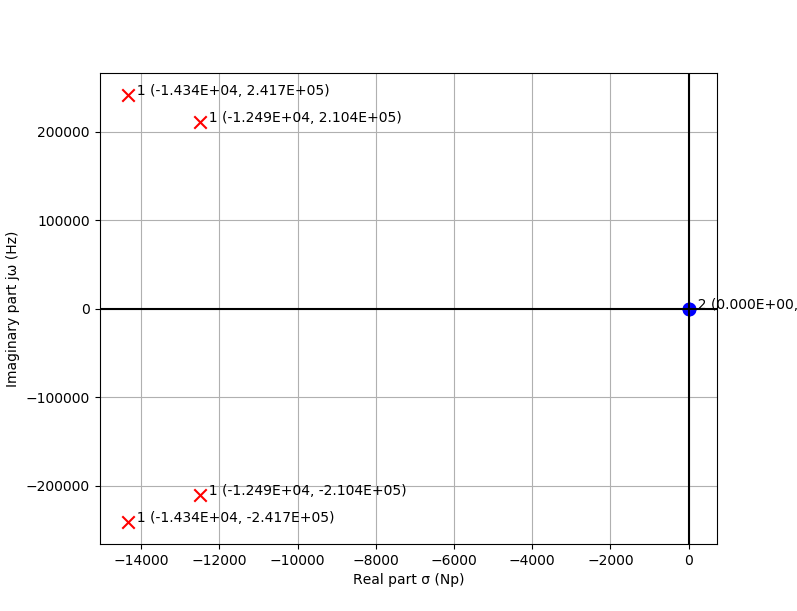
\includegraphics{../EJ2/Recursos/CHEBY_POLES}       
    }
    \caption{Polos y ceros de la transferencia}
    \label{fig:CHEBY_POLES}
\end{figure}

Se pueden observar los diagrams de atenuaci\'on y fase de la transferencia en la Figura \ref{fig:CHEBY_BODE}.
\begin{figure}[H]
    \centering
    \begin{tabular}{c c}
        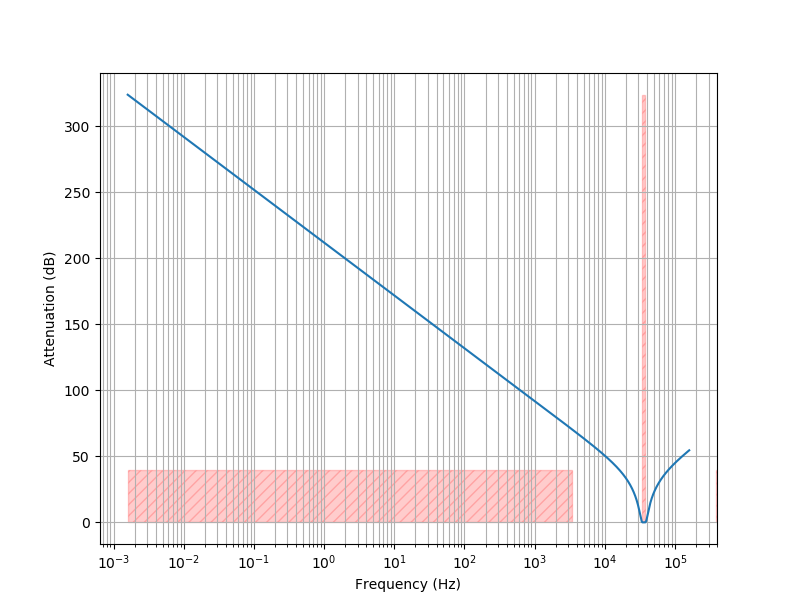
\includegraphics[scale=0.3]{../EJ2/Recursos/CHEBY_ATT} &
        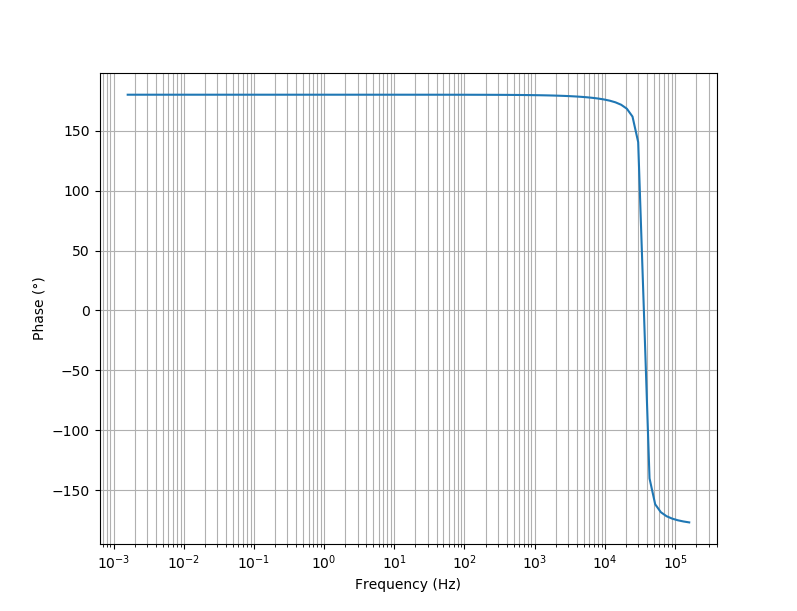
\includegraphics[scale=0.3]{../EJ2/Recursos/CHEBY_PHASE} \\        
    \end{tabular}
    \caption{Diagrams de atenuaci\'on y fase de la transferencia}
    \label{fig:CHEBY_BODE}
\end{figure}

Sin embargo, debido a que la celda a implementar tiene una transferencia que es de segundo orden, es necesario separar la transferencia obtenida en 2 transferencias de menor orden. De esta forma es posible calcular los componentes que se requieren para cada etapa. Este an\'alisis, junto con las respectivas simulaciones, es tratado en las siguientes secciones

Al separar la transferencia en 2 etapas de segundo orden se obtiene el resultado que se observa en \ref{eq:CHEBY_SOS}

\begin{equation}
    H(s) = \num{1.68e9}\frac{s}{s^2 + \num{28.68e3}s + \num{58.61e9}}\cdot \frac{s}{s^2 + \num{24.98e3}s + \num{44.44e9}}
    \label{eq:CHEBY_SOS}
\end{equation}

\subsubsection{$1^\circ$ etapa}
Como se debe hacer un filtro para bajas se\~nales, se prioriza que la primera etapa tenga mayor ganancia que la segunda. Sin embargo tambi\'en se debe tener en cuenta que, de preferencia, la segunda etapa no debe atenuar y adem\'as debe poder realizarse la etapa con componentes de valores razonables.
Con esas consideraciones, se dise\~na la etapa para que cumpla con la transferencia que se muestra en \ref{eq:1_TRANFER}

\begin{equation}
    H(s) = \frac{\num{42e3}\cdot s}{s^2 + \num{24.98e3}s + \num{44.44e9}}
    \label{eq:1_TRANFER}
\end{equation}
En base a las expresiones para los componentes mostradas en el an\'alisis, y en las caracter\'isticas que se obtienen de la transferencia que se observan en la Tabla \ref{tab:1_TRANSFER_CHAR}, se obtienen para esta etapa los valores de componentes mostrados en la Tabla \ref{tab:1_VALUES}
\begin{table}[H]
    \centering
    \resizebox{0.3\textwidth}{!}{%
    \begin{tabular}{cc}
    \hline
    \multicolumn{2}{c}{Primera etapa} \\ \hline
    $H_P$ (Veces) & 1.681 \\
    Q & 8.44 \\
    $\omega_0$ (rad/s)& $\num{2.11e5}$ \\ \hline
    \end{tabular}%
    }
    \caption{Caracter\'isticas de la primera etapa}
    \label{tab:1_TRANSFER_CHAR}
\end{table}
\begin{table}[H]
    \centering
    \resizebox{0.3\textwidth}{!}{%
    \begin{tabular}{cc}
    \hline
    \multicolumn{2}{c}{Valores de componentes} \\ \hline
    R1/a & $85.56 K\Omega$ \\
    R1/(1-a) & $5075\Omega$ \\
    R2 & $43.12K\Omega$ \\
    $K\cdot R$ & $1.54K\Omega$ \\
    $(1-K)\cdot$ R & $8.46K\Omega$ \\
    C & 330pF \\ \hline
    \end{tabular}%
    }
    \caption{Valores de componentes para la primera etapa}
    \label{tab:1_VALUES}
\end{table}
Se muestra en la Figura \ref{fig:1_HIST} un histograma donde se puede observar la variacion de la frecuencia a la que se encuentran los polos del sistema con respecto a la variaci\'on debida a la tolerancia de los componentes.
\begin{figure}[H]
    \centering
    \resizebox{\textwidth}{!}{%        
        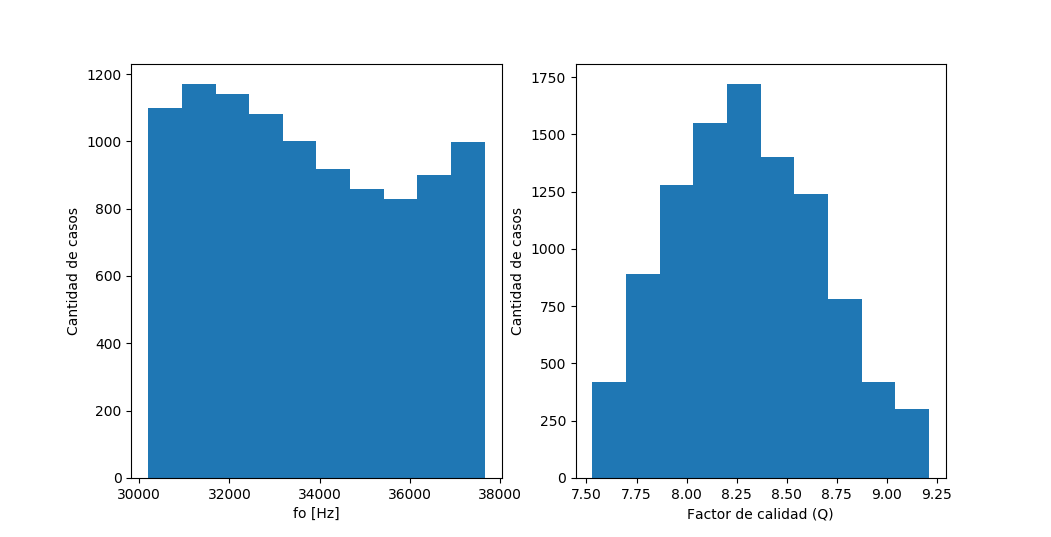
\includegraphics{../EJ2/Recursos/HIST_FIRST}       
    }
    \caption{Histograma de la primera etapa}
    \label{fig:1_HIST}
\end{figure}
Por \'ultimo se muestra en la Figura \ref{fig:FIRST_LT_VS_TEO} una comparaci\'on entre los resultados obtenidos en LTSpice por medio del an\'alisis Monte Carlo y la curva te\'orica de la transferencia esperada.
\begin{figure}[H]
    \centering
    \resizebox{0.8\textwidth}{!}{%        
        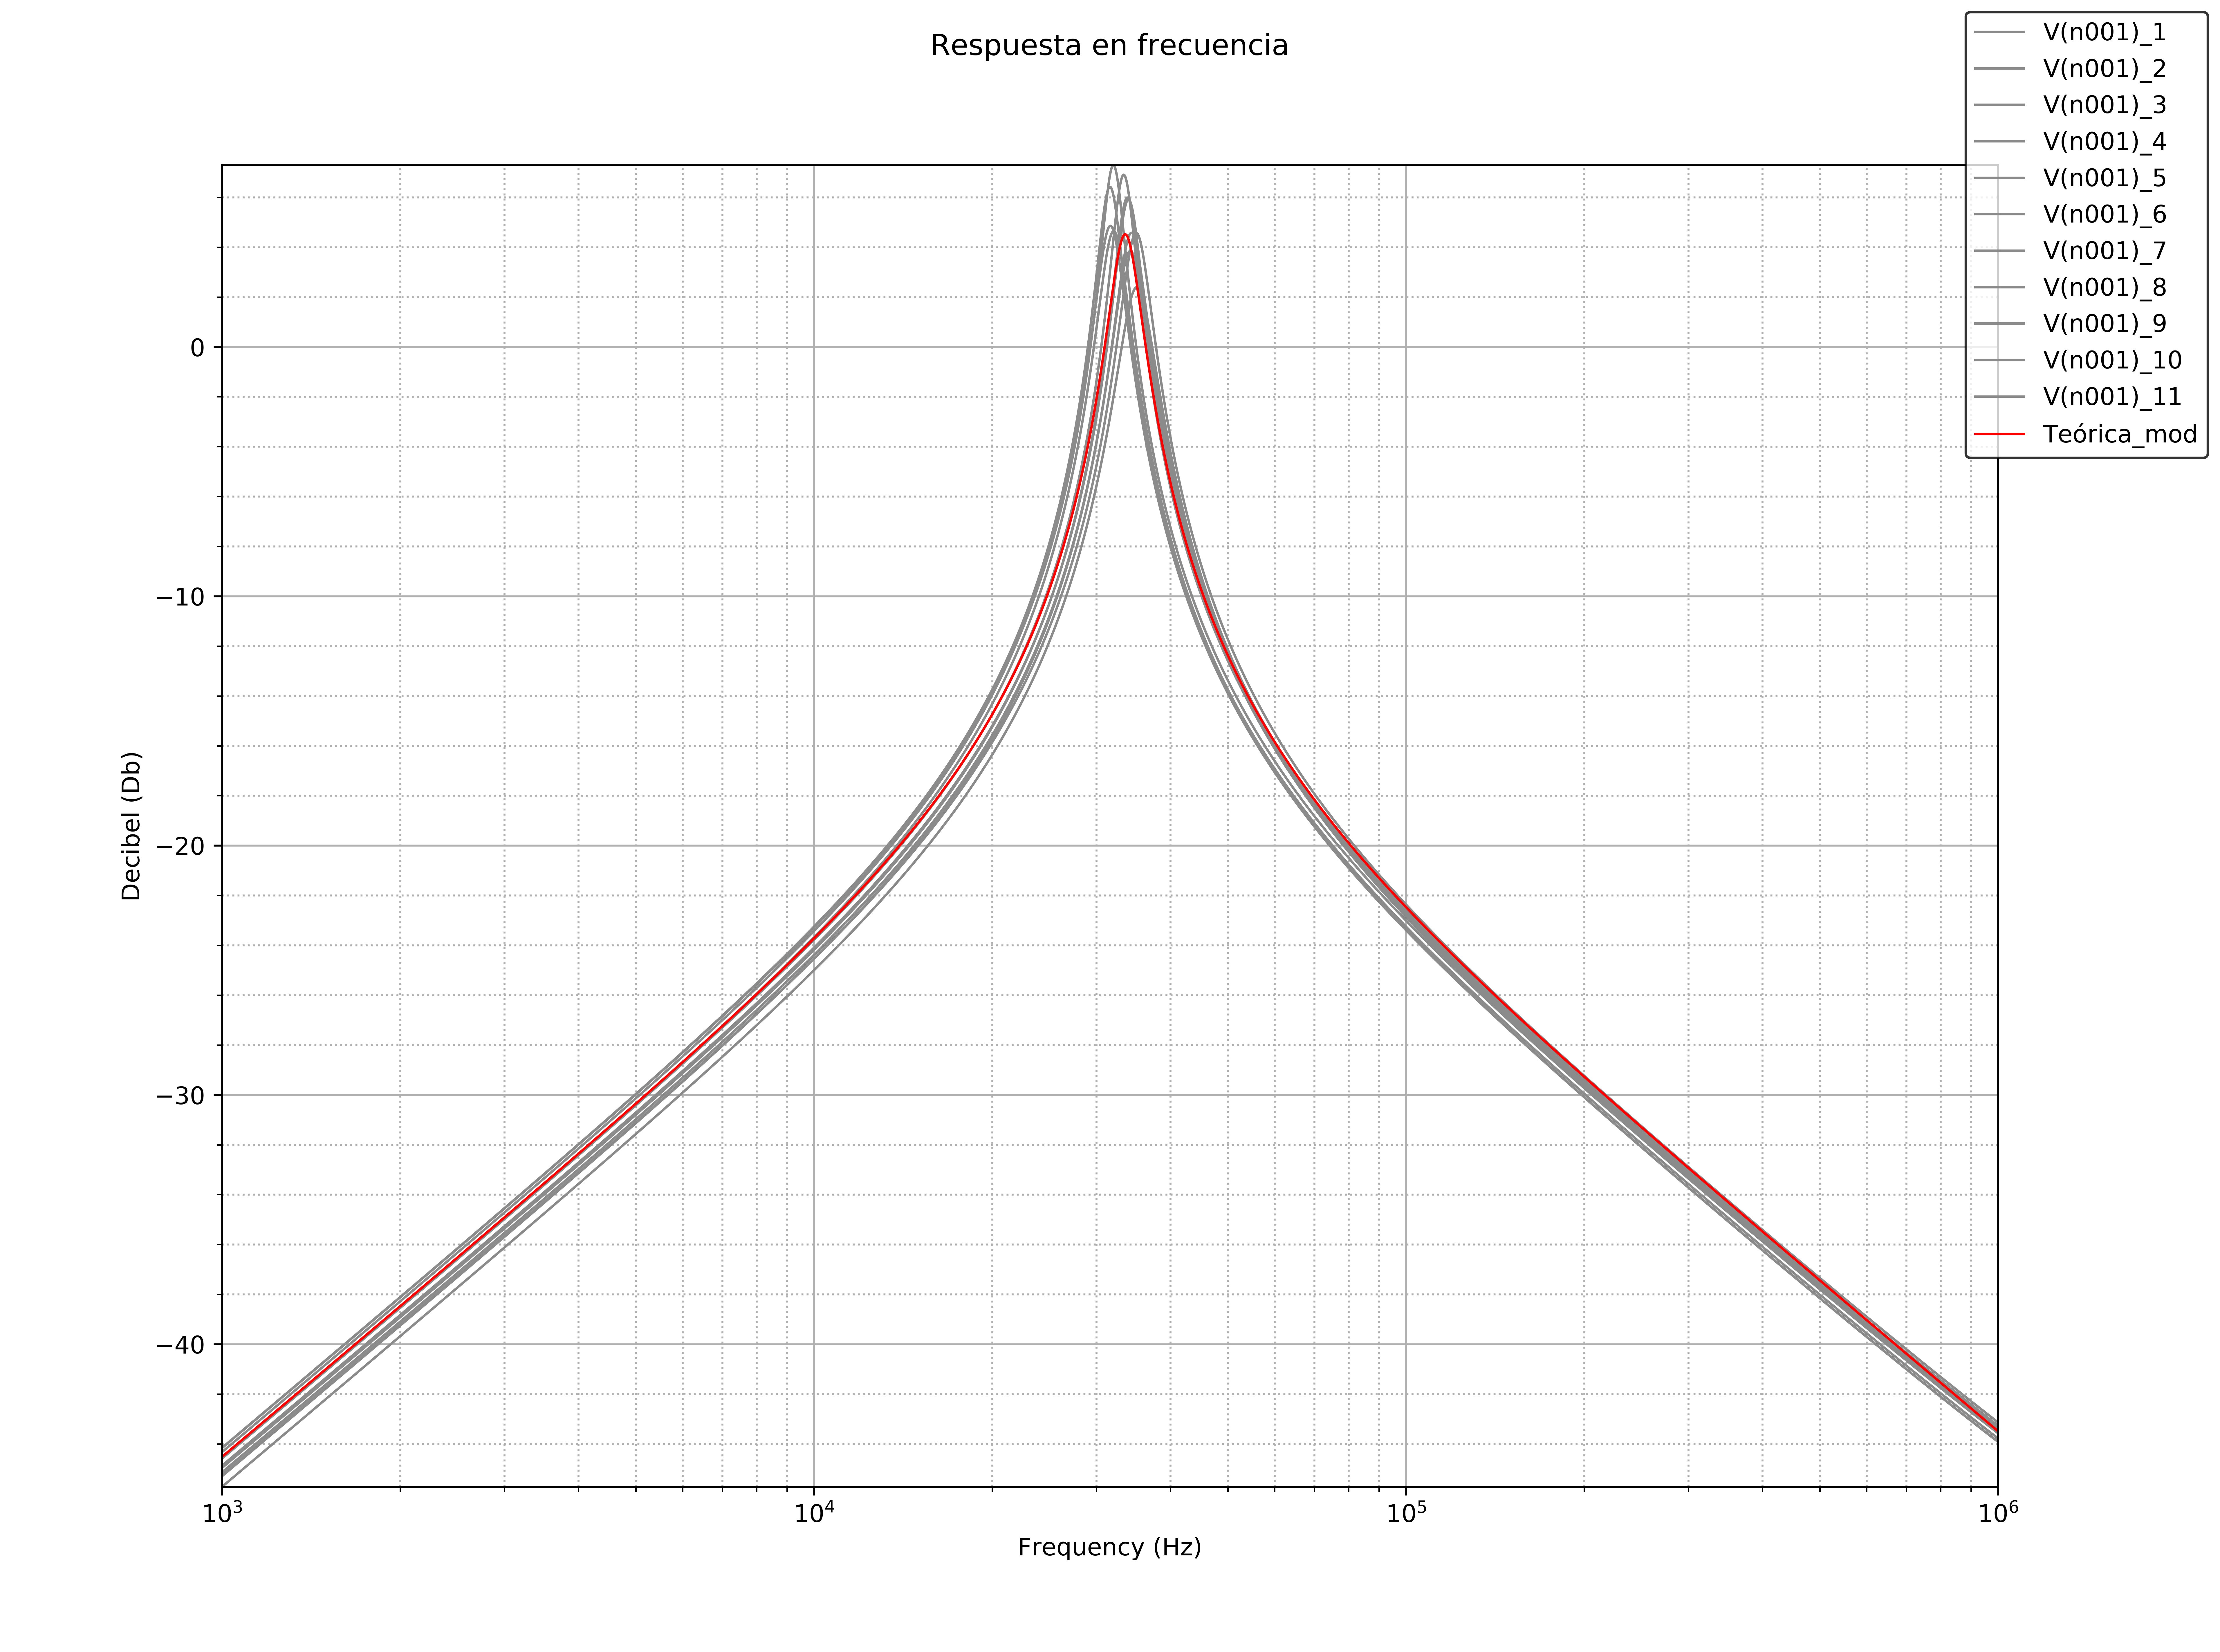
\includegraphics{../EJ2/Recursos/FIRST_LT_VS_TEO}       
    }
    \caption{Comparaci\'on con simulaciones de la primera etapa}
    \label{fig:FIRST_LT_VS_TEO}
\end{figure}

\subsubsection{$2^\circ$ etapa}
Se dise\~na la etapa para que cumpla con la transferencia que se muestra en \ref{eq:2_TRANFER}

\begin{equation}
    H(s) = \frac{\num{39.9e3}\cdot s}{s^2 + \num{28.68e3}s + \num{58.61e9}}
    \label{eq:1_TRANFER}
\end{equation}
En base a las expresiones para los componentes mostradas en el an\'alisis, y en las caracter\'isticas que se obtienen de la transferencia que se observan en la Tabla \ref{tab:2_TRANSFER_CHAR}, se obtienen para esta etapa los valores de componentes mostrados en la Tabla \ref{tab:2_VALUES}
\begin{table}[H]
    \centering
    \resizebox{0.3\textwidth}{!}{%
    \begin{tabular}{cc}
    \hline
    \multicolumn{2}{c}{Segunda etapa} \\ \hline
    $H_P$ (Veces) &1.391 \\
    Q & 8.44 \\
    $\omega_0$ (rad/s)& $\num{2.42e5}$ \\ \hline
    \end{tabular}%
    }
    \caption{Caracter\'isticas de la segunda etapa}
    \label{tab:2_TRANSFER_CHAR}
\end{table}
\begin{table}[H]
    \centering
    \resizebox{0.3\textwidth}{!}{%
    \begin{tabular}{cc}
    \hline
    \multicolumn{2}{c}{Valores de componentes} \\ \hline
    R1/a & $63.68 K\Omega$ \\
    R1/(1-a) & $3070\Omega$ \\
    R2 & $26.36K\Omega$ \\
    $K\cdot R$ & $1.54K\Omega$ \\
    $(1-K)\cdot$ R & $8.46K\Omega$ \\
    C & 470pF \\ \hline
    \end{tabular}%
    }
    \caption{Valores de componentes para la segunda etapa}
    \label{tab:2_VALUES}
\end{table}
Se muestra en la Figura \ref{fig:2_HIST} un histograma donde se puede observar la variaci\'on de la frecuencia a la que se encuentran los polos del sistema con respecto a la variaci\'on debida a la tolerancia de los componentes.
\begin{figure}[H]
    \centering
    \resizebox{\textwidth}{!}{%        
        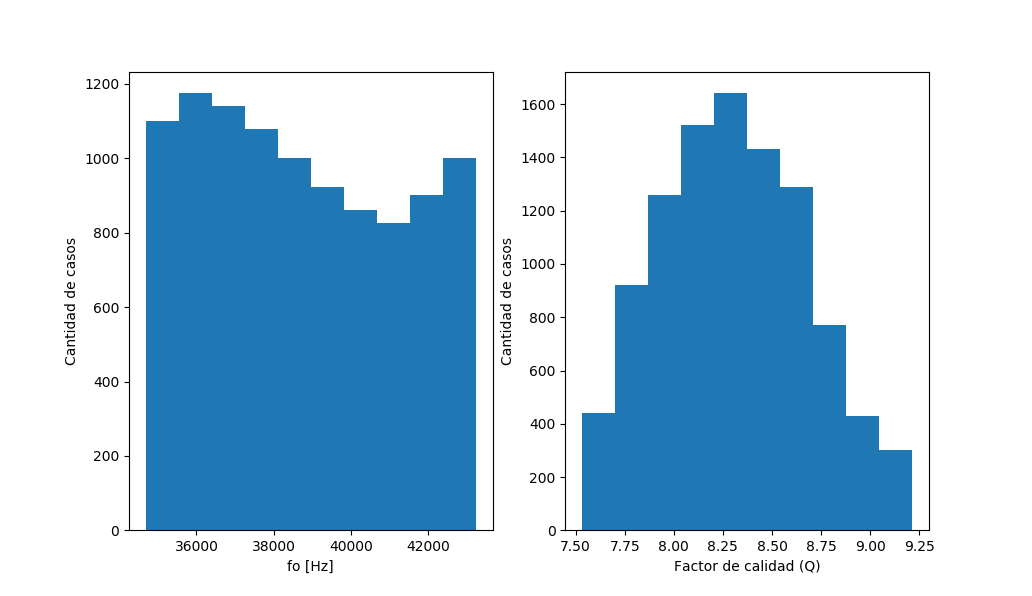
\includegraphics{../EJ2/Recursos/HIST_SECOND}       
    }
    \caption{Histograma de la segunda etapa}
    \label{fig:2_HIST}
\end{figure}


Por \'ultimo se muestra en la Figura \ref{fig:FIRST_LT_VS_TEO} una comparaci\'on entre los resultados obtenidos en LTSpice por medio del an\'alisis Monte Carlo y la curva te\'orica de la transferencia esperada.
\begin{figure}[H]
    \centering
    \resizebox{0.8\textwidth}{!}{%        
        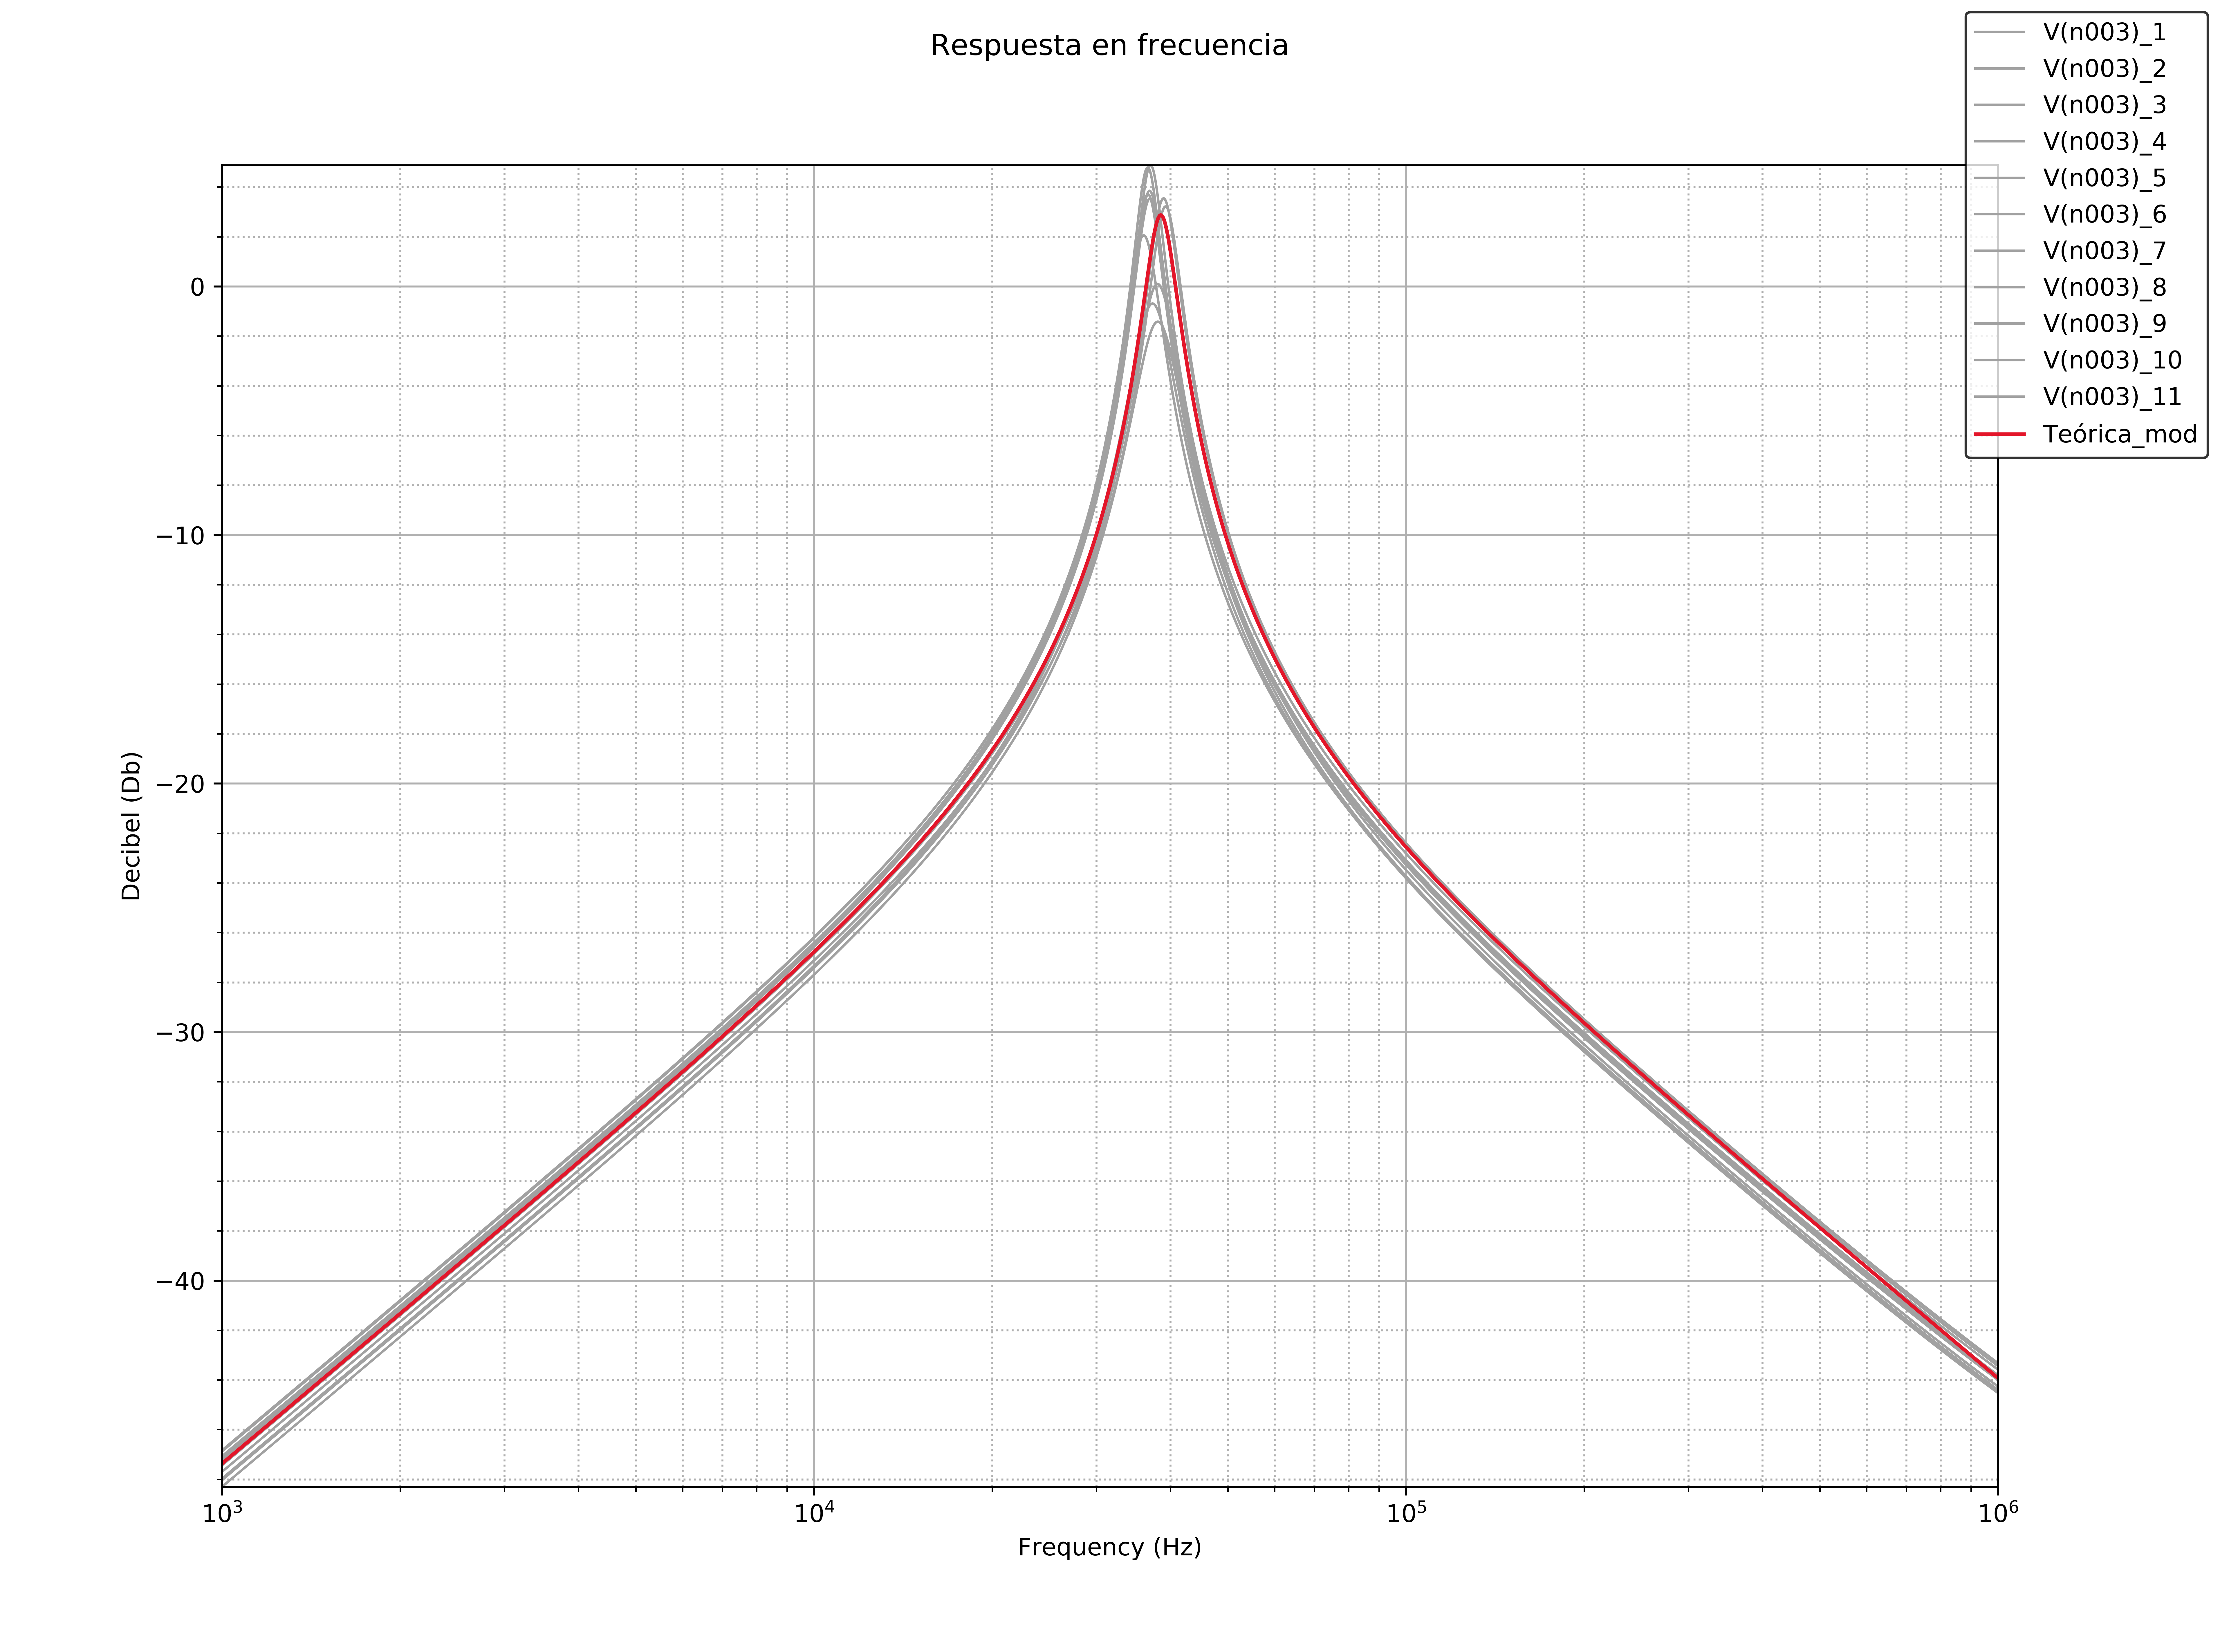
\includegraphics{../EJ2/Recursos/SECOND_LT_VS_TEO}       
    }
    \caption{Comparaci\'on con simulaciones de la segunda etapa}
    \label{fig:FIRST_LT_VS_TEO}
\end{figure}

\subsubsection{Simulaciones en cascada}
Se realizan simulaciones Monte Carlo en LTSpice de las 2 etapas anteriores conectadas en cascada para verificar que tanto la la transferencia cumpla con la pantilla, como que la impedancia de entrada se mantenga en los randos especificados, al menos en las simulaciones.

Se muestra en las Figuras \ref{fig:MC_MOD} y \ref{fig:MC_PHASE} las simulaciones de m\'odulo y fase de la respuesta en frecuencia del circuito.
\begin{figure}[H]
    \centering
    \resizebox{0.8\textwidth}{!}{%        
        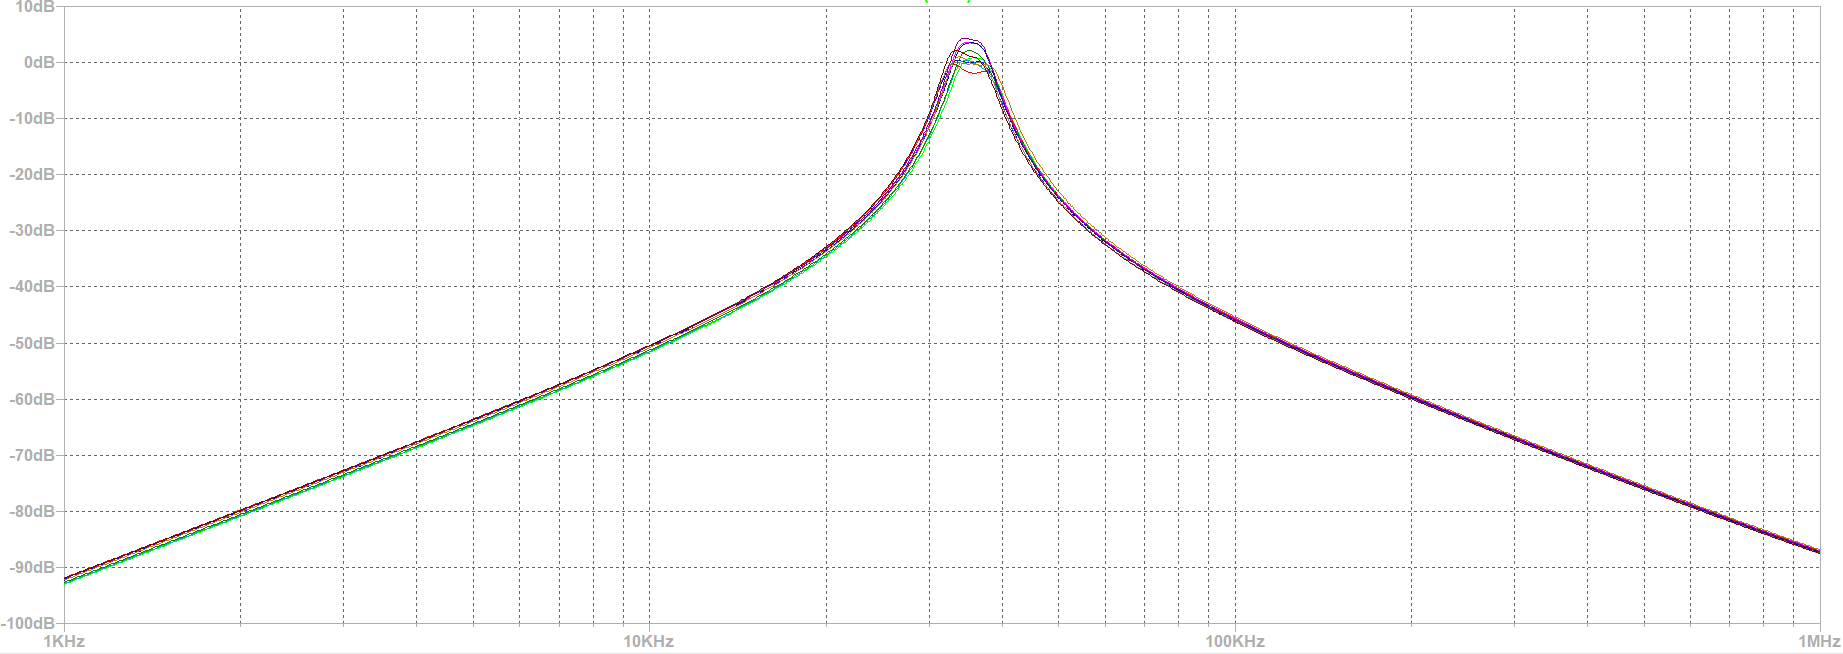
\includegraphics{../EJ2/Recursos/MC_MOD}       
    }
    \caption{Simulaci\'on del m\'odulo de la transferencia del filtro}
    \label{fig:MC_MOD}
\end{figure}
\begin{figure}[H]
    \centering
    \resizebox{0.8\textwidth}{!}{%        
        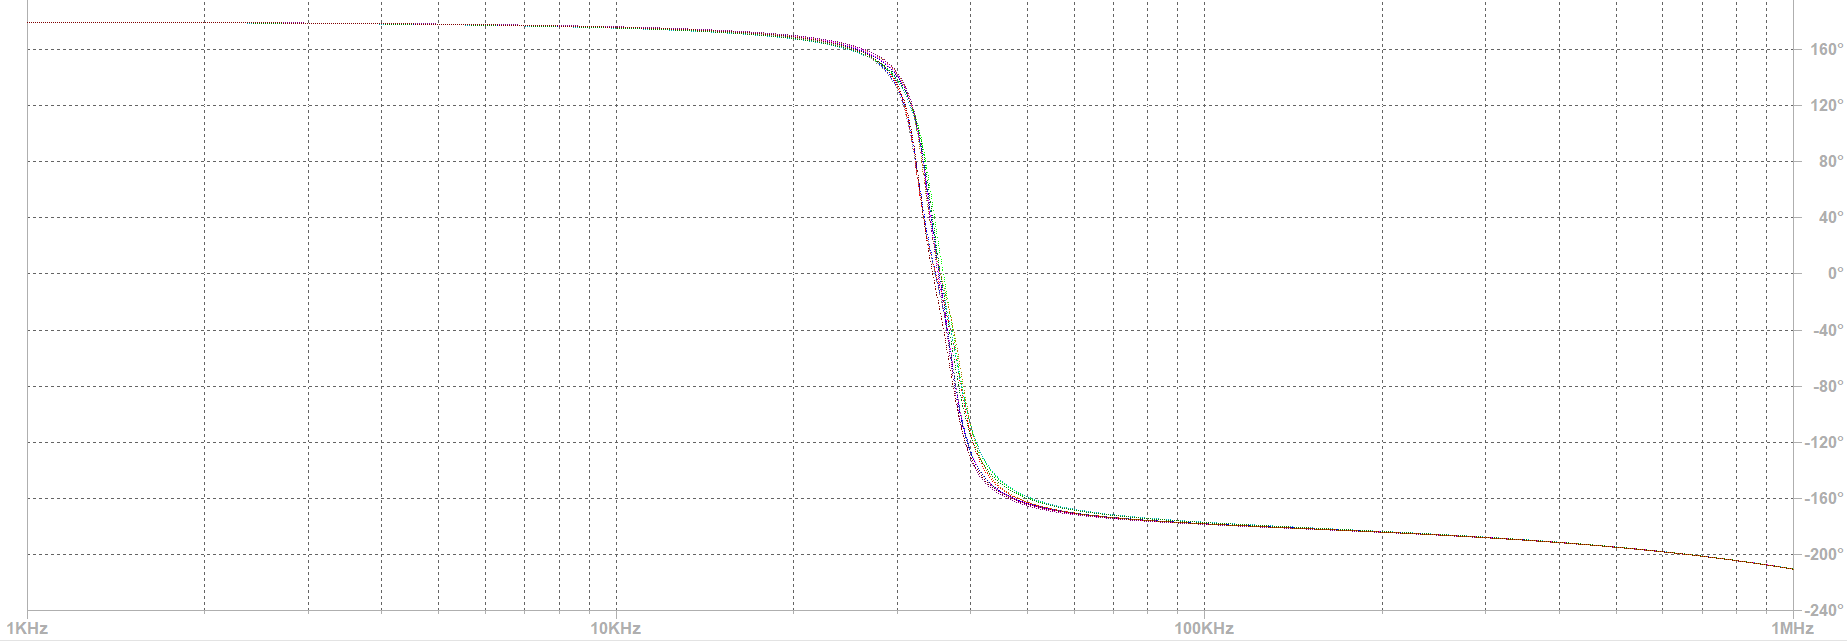
\includegraphics{../EJ2/Recursos/MC_PHA}       
    }
    \caption{Simulaci\'on del fase de la transferencia del filtro}
    \label{fig:MC_PHASE}
\end{figure}
Se muestra en la Figura \ref{fig:VERIFY} un aumento sobre la banda de paso, con el fin de verificar que se cumple la plantilla en ese rango de frecuencias.
\begin{figure}[H]
    \centering
    \resizebox{0.8\textwidth}{!}{%        
        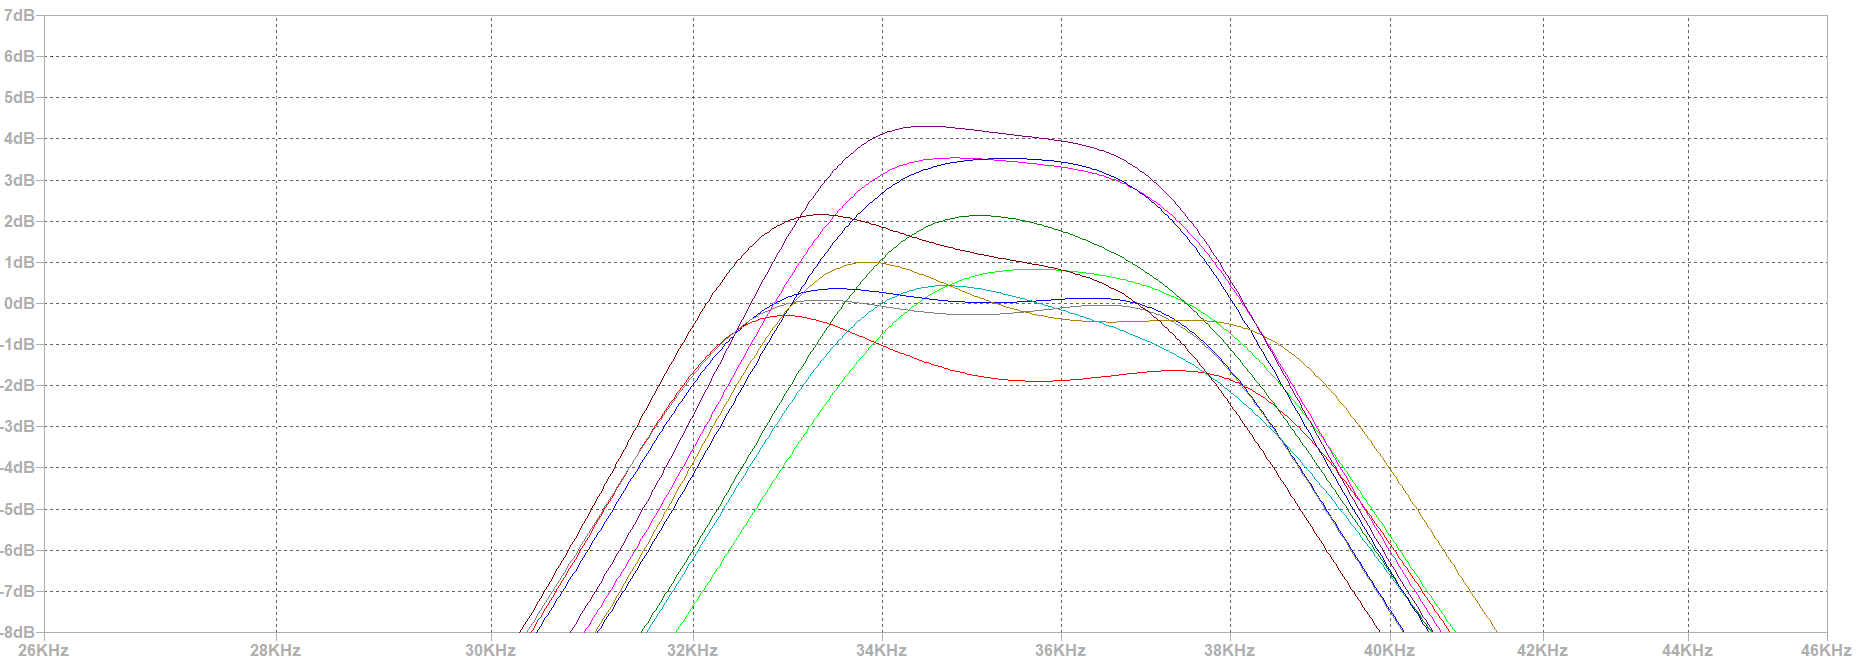
\includegraphics{../EJ2/Recursos/MC_VER}       
    }
    \caption{Verificaci\'on de plantilla en la banda de paso}
    \label{fig:VERIFY}
\end{figure}
Puede observarse que, en todos los casos se ve una frecuencia de corte de aproximadamente 36KHz, donde la atenuaci\'on al alejarse una decada de esa frecuencia es mayor a 40dB, que son par\'ametro de dise\~no, y que en la banda pasante, la atenuaci\'on nunca supera los 3dB. Sin embargo se observa que para algunos casos, la ganancia en la banda pasante es superior a 0dB. Este efecto no es deseado, pero en la mayor\'ia de los casos la ganancia no supera los 3dB(2veces) con lo que se supone este efecto de caracter despreciable y no se realizan correcciones sobre este ni en las simulaciones ni en el dise\~no f\'isico del circuito.


Se puede observar adem\'as, la simulacion de la impedancia de entrada del filtro en la Figura \ref{fig:ZIN_SIST}
\begin{figure}[H]
    \centering
    \resizebox{0.8\textwidth}{!}{%        
        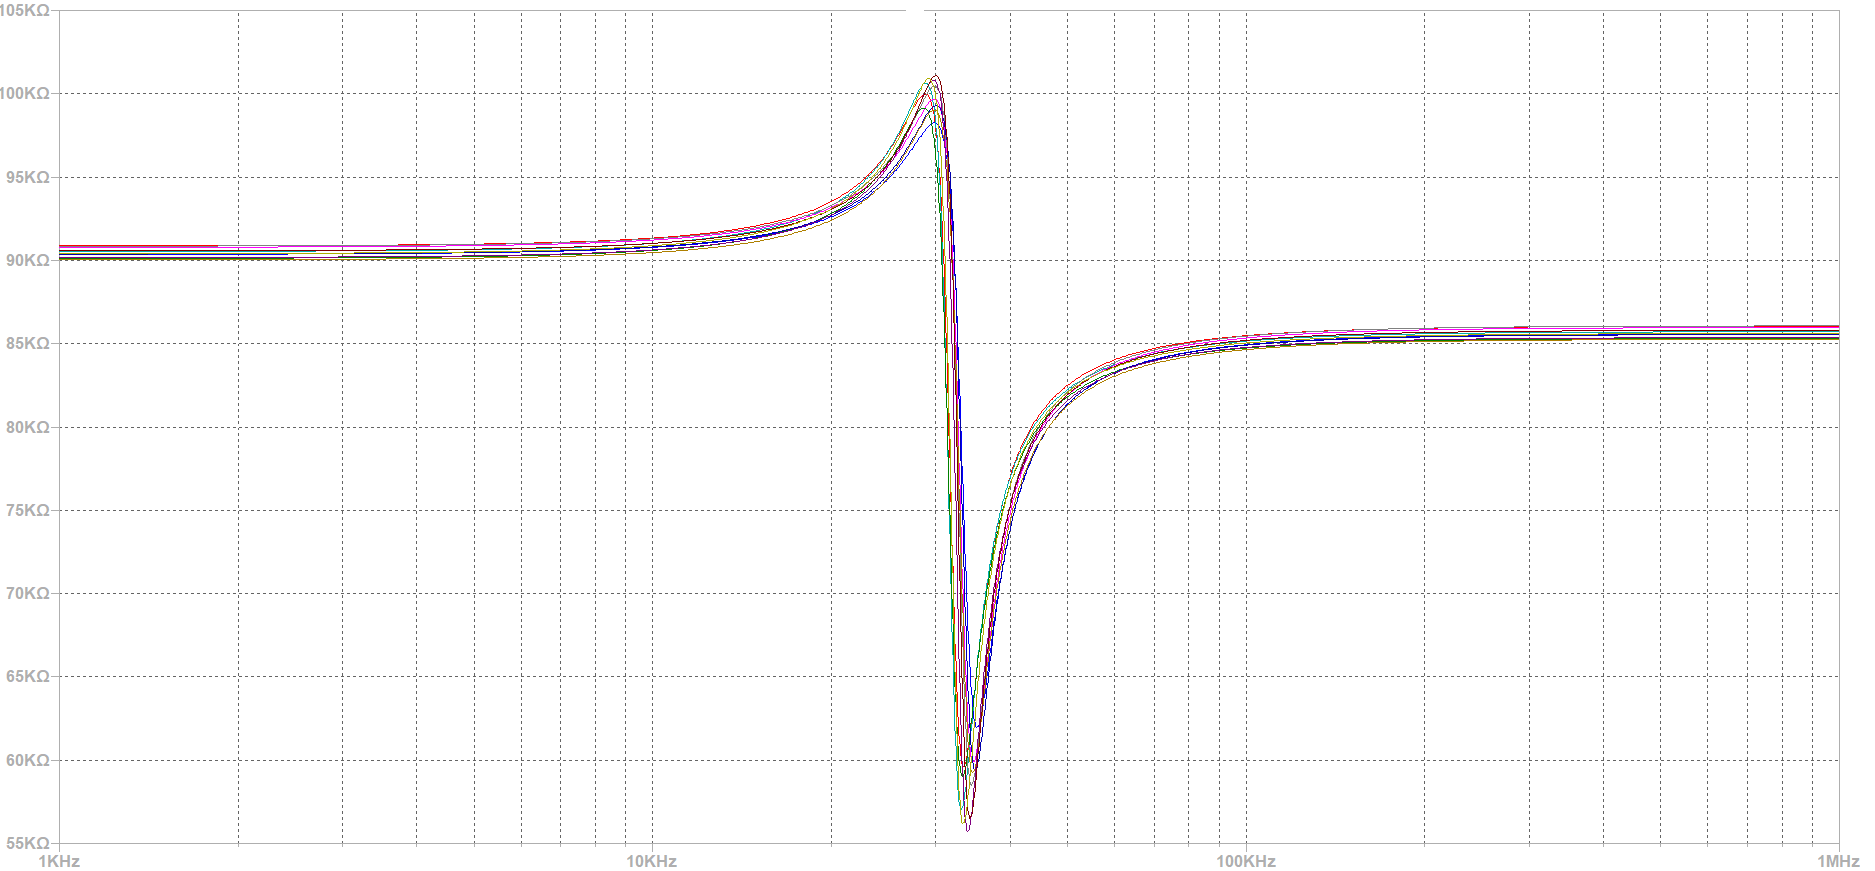
\includegraphics{../EJ2/Recursos/ZIN}       
    }
    \caption{Simulaci\'on de la impedancia de entrada del sistema}
    \label{fig:ZIN_SIST}
\end{figure}

\subsubsection{Mediciones y comparaciones}
En esta secci\'on se presenta la comparaci\'on entre las curvas te\'oricas, simuladas y medidas de el m\'odulo de la transferencia de las 2 etapas pasabanda por separado(Figuras \ref{fig:FIRST_LT_VS_TEO_VS_MED} y \ref{fig:SECOND_LT_VS_TEO_VS_MED}), el m\'odulo y la fase de la transferencia del filtro completo(Figura \ref{fig:COMP_BODE}) y la impedancia de entrada del filtro completo (Figura \ref{fig:ZIN}).
\begin{figure}[H]
    \centering
    \resizebox{0.8\textwidth}{!}{%        
        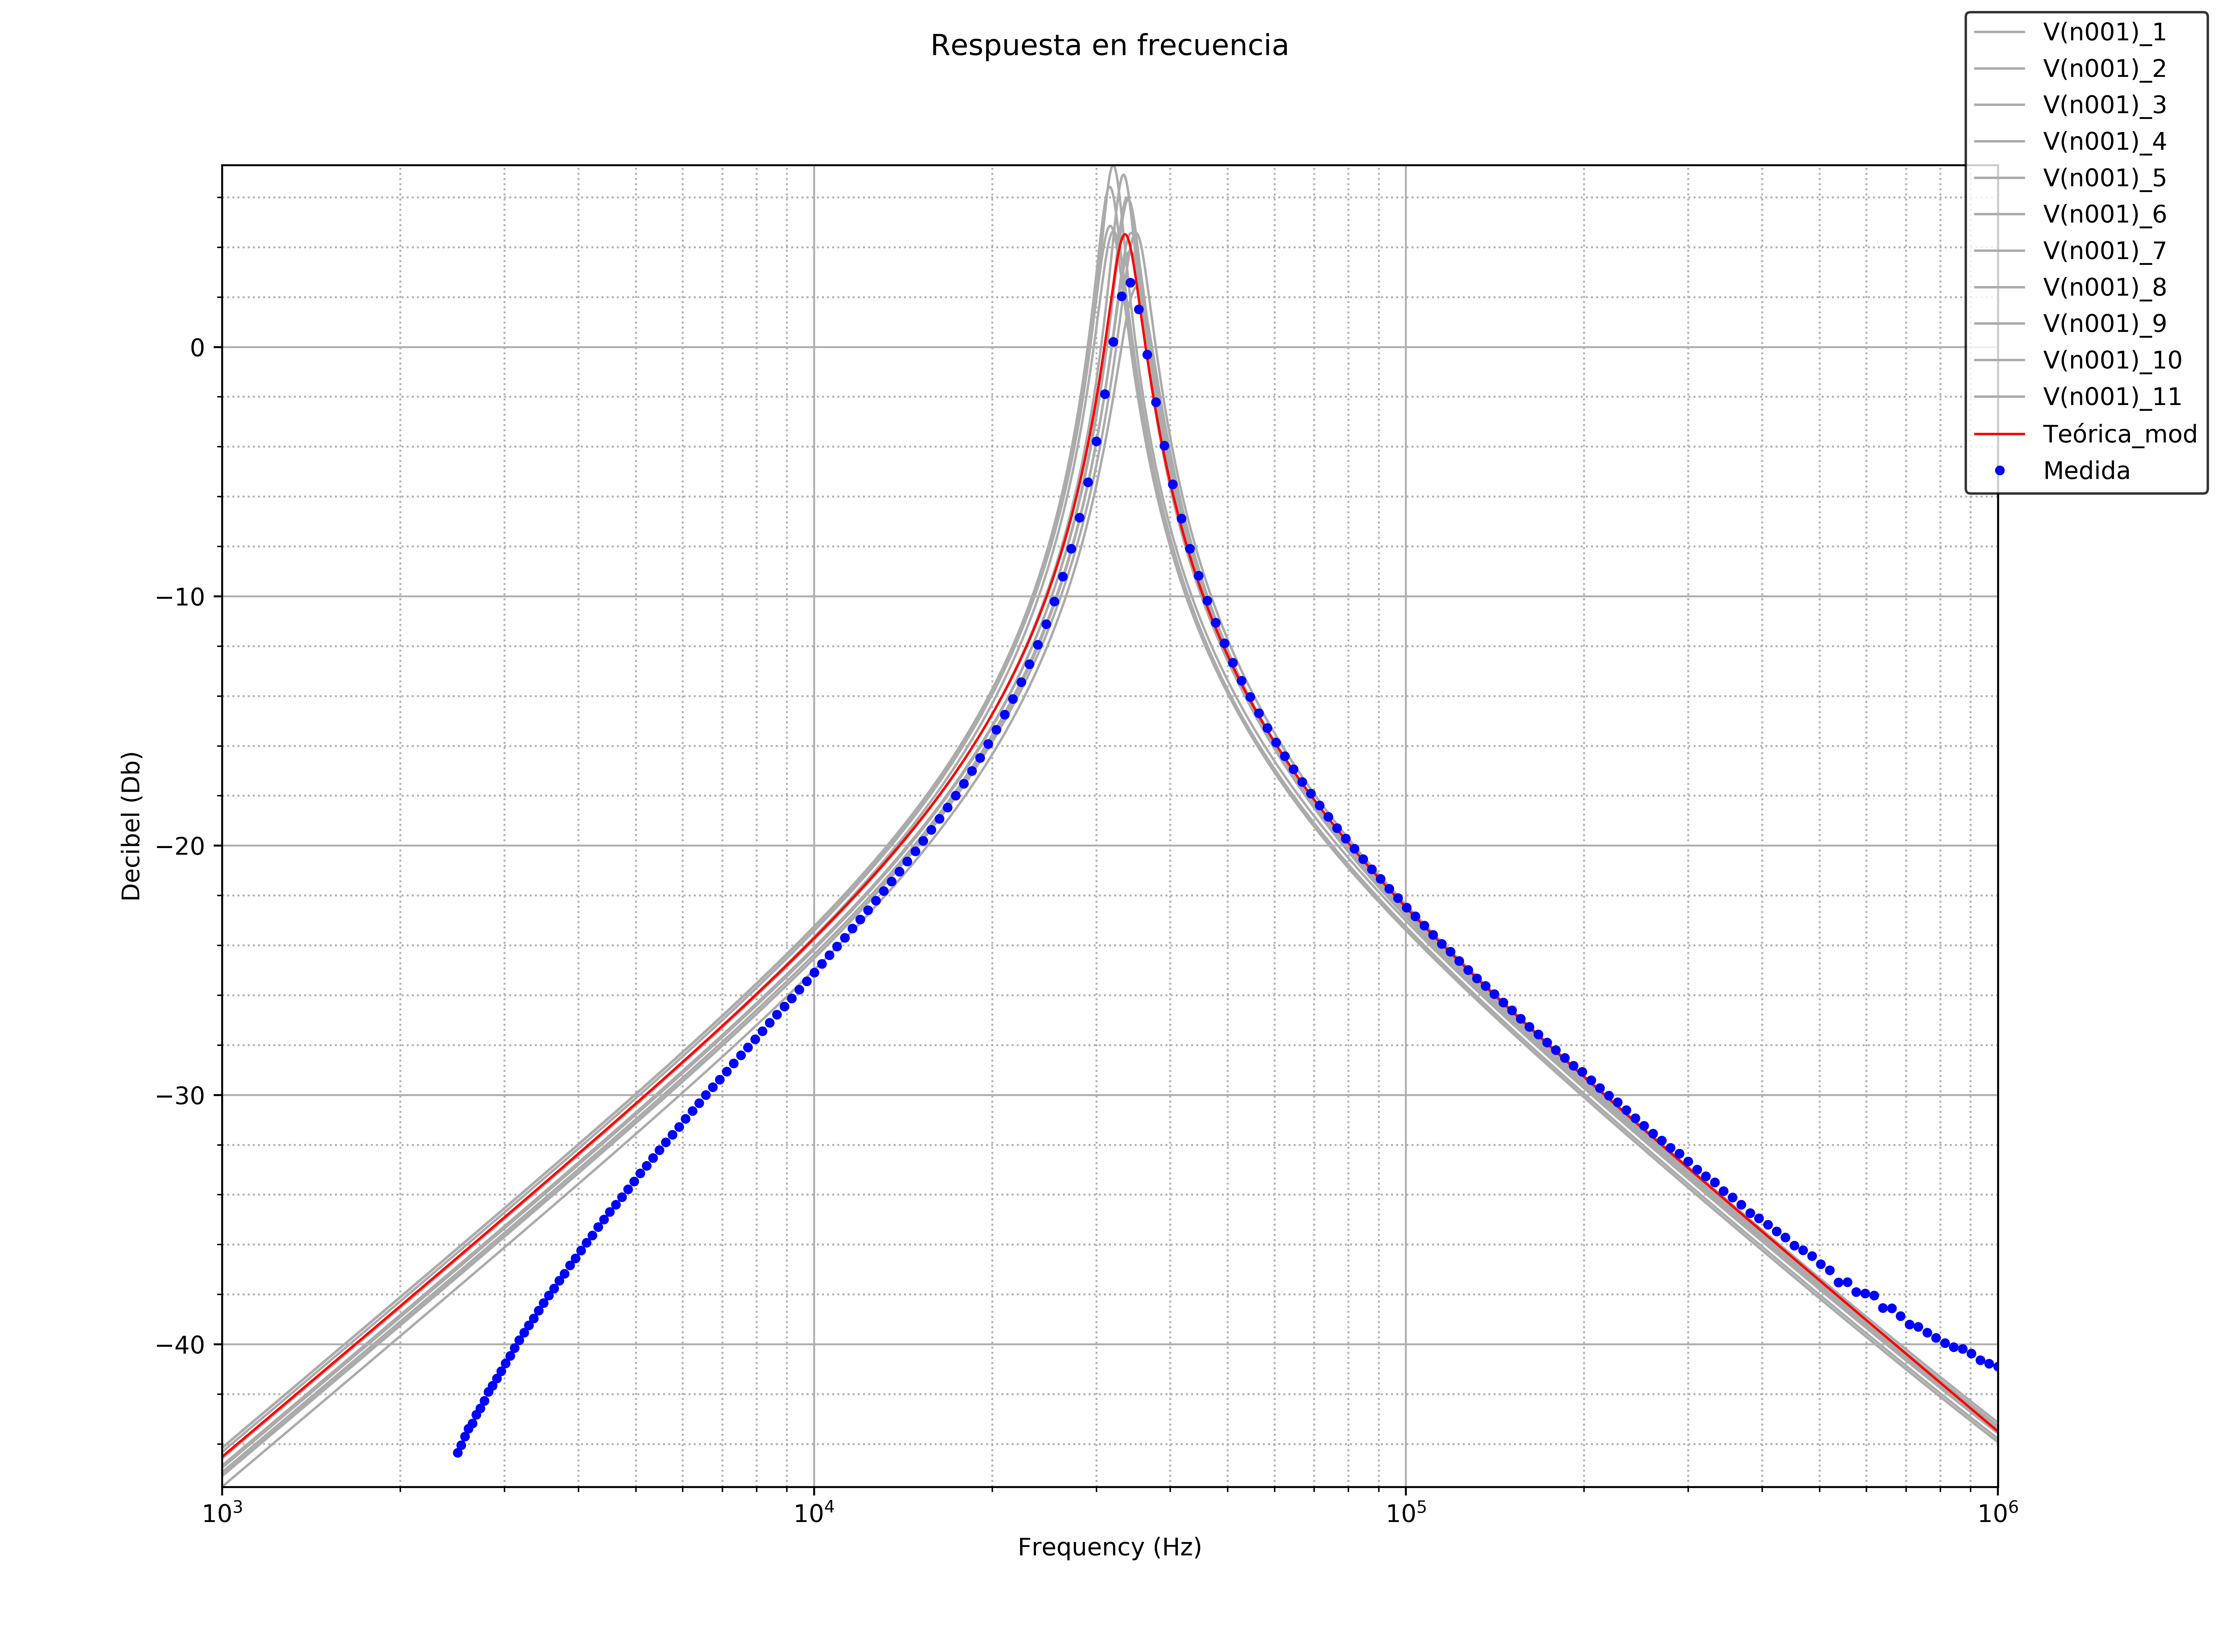
\includegraphics{../EJ2/Recursos/FIRST_LT_VS_TEO_VS_MED}       
    }
    \caption{Comparaci\'on de curvas para la primera etapa}
    \label{fig:FIRST_LT_VS_TEO_VS_MED}
\end{figure}
\begin{figure}[H]
    \centering
    \resizebox{0.8\textwidth}{!}{%        
        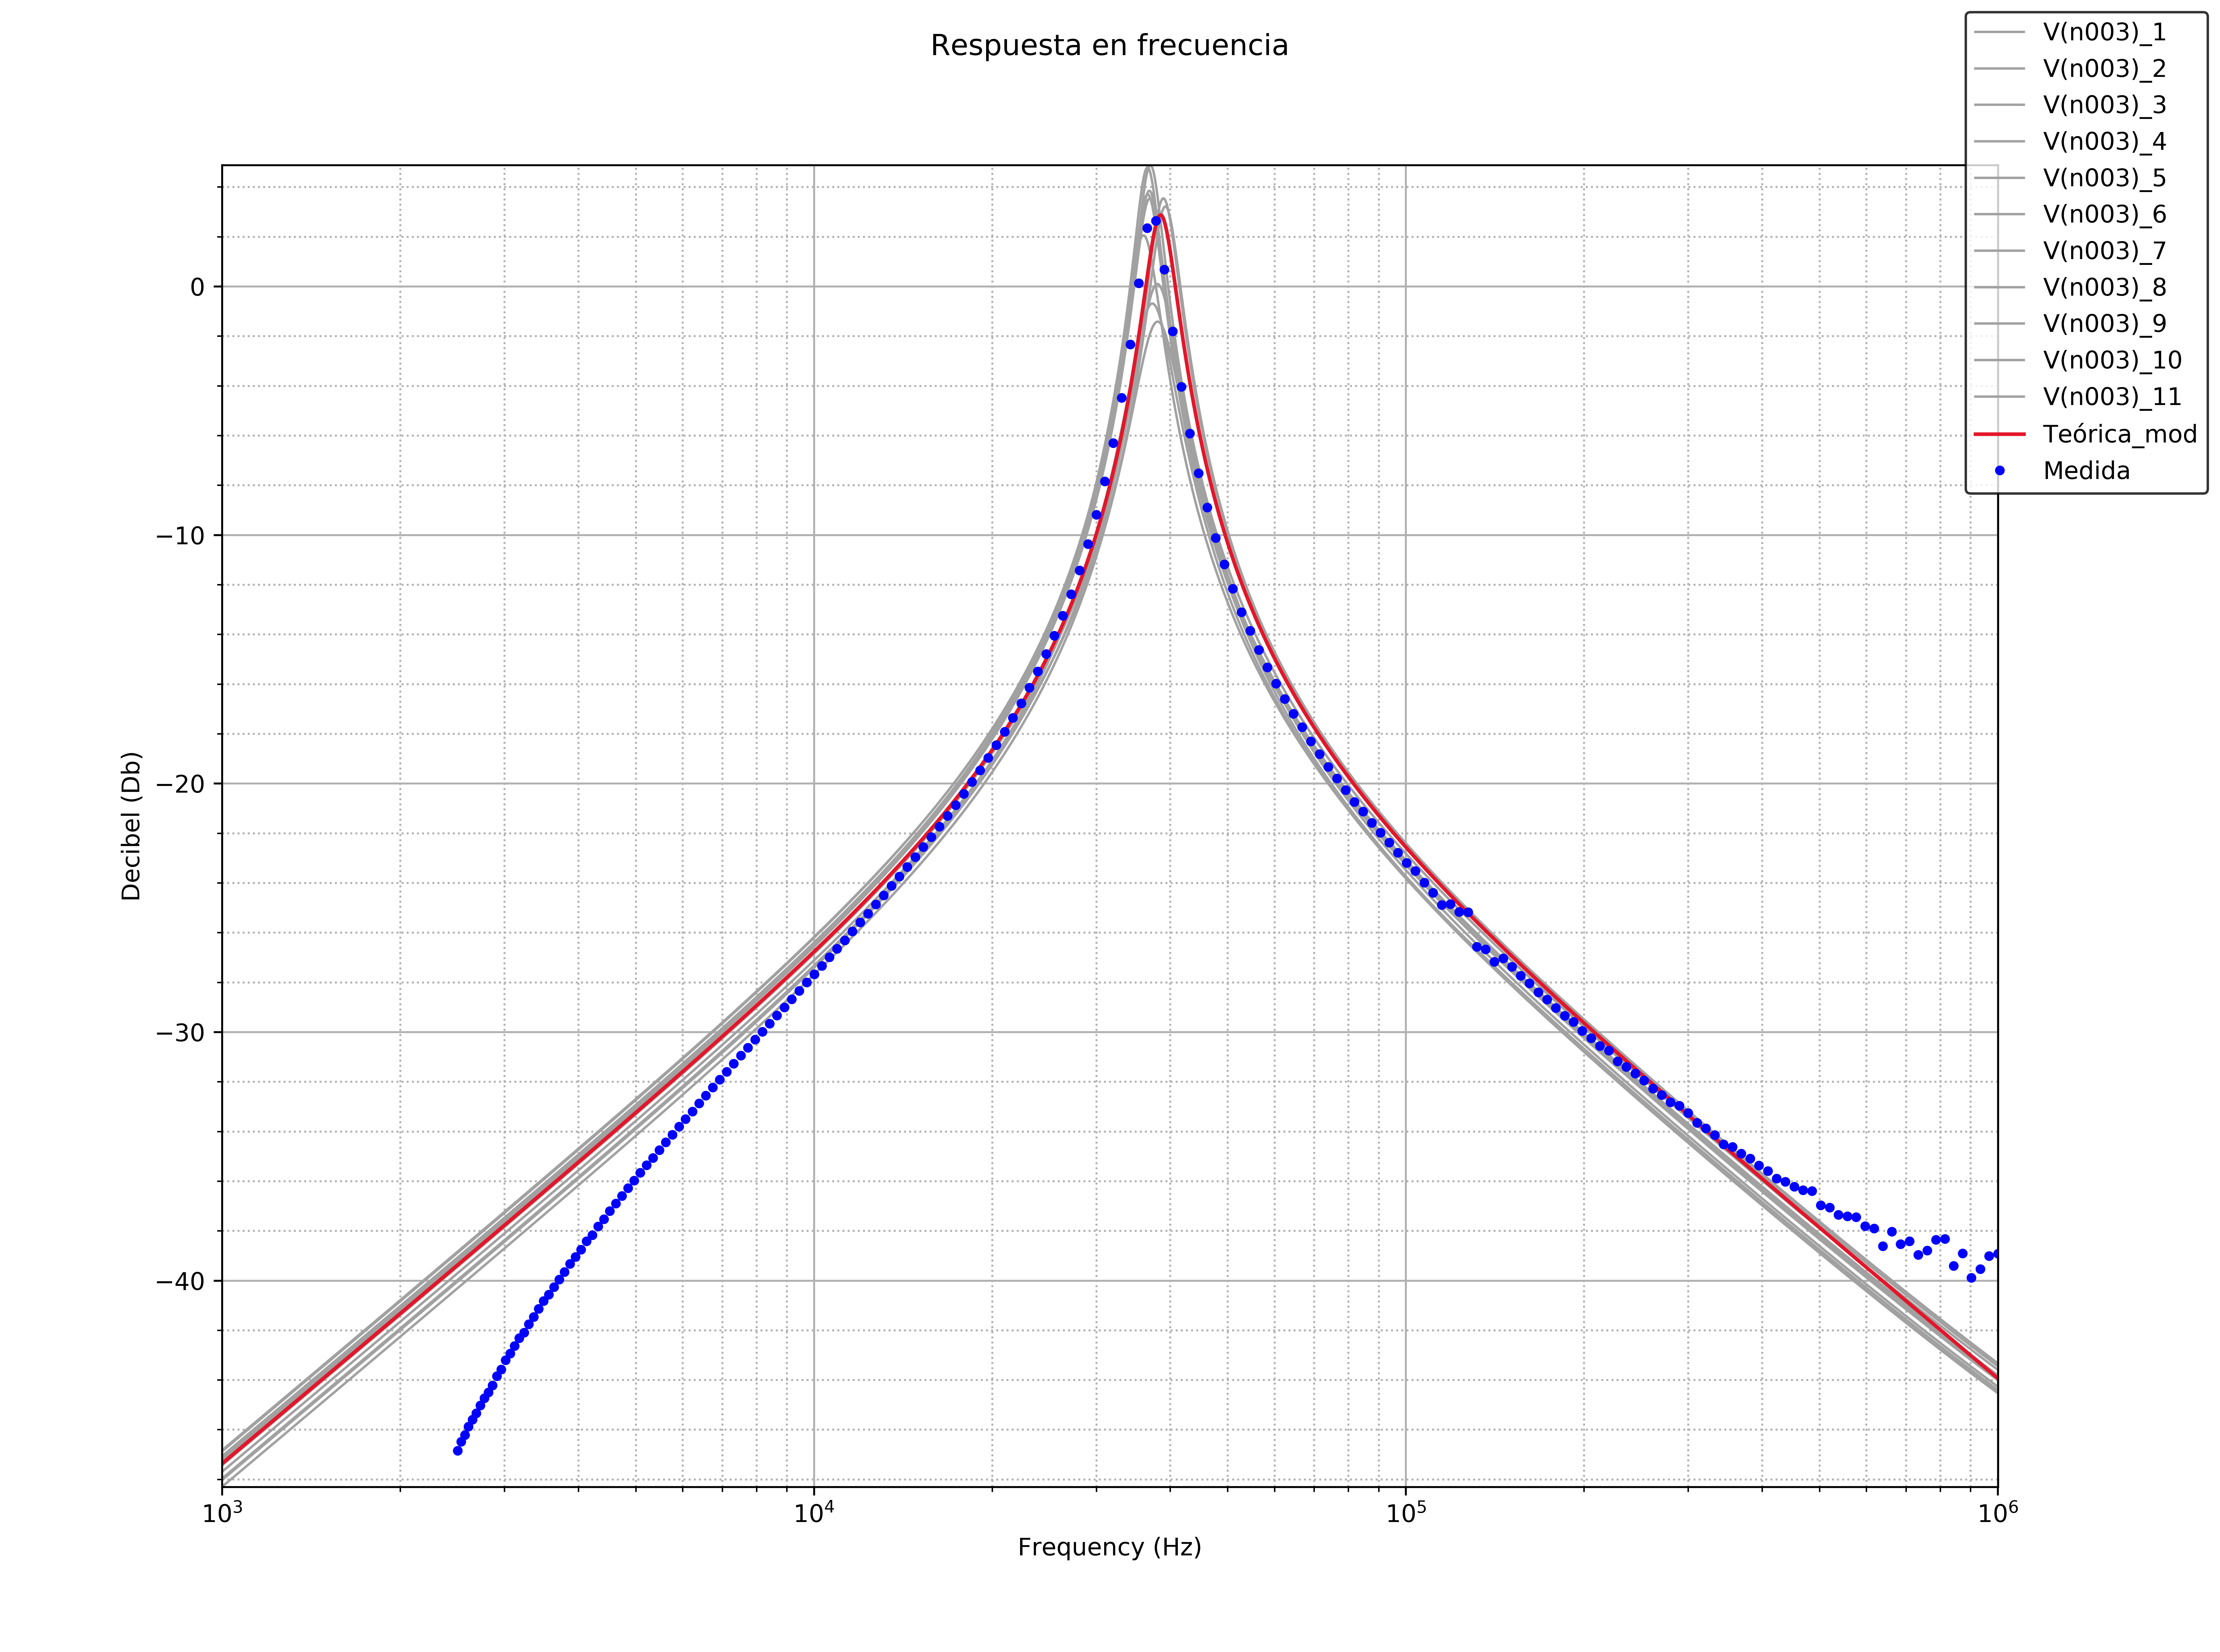
\includegraphics{../EJ2/Recursos/SECOND_LT_VS_TEO_VS_MED}       
    }
    \caption{Comparaci\'on de curvas para la segunda etapa}
    \label{fig:SECOND_LT_VS_TEO_VS_MED}
\end{figure}
\begin{figure}[H]
    \centering
    \resizebox{0.8\textwidth}{!}{% 
    \begin{tabular}{c c}
        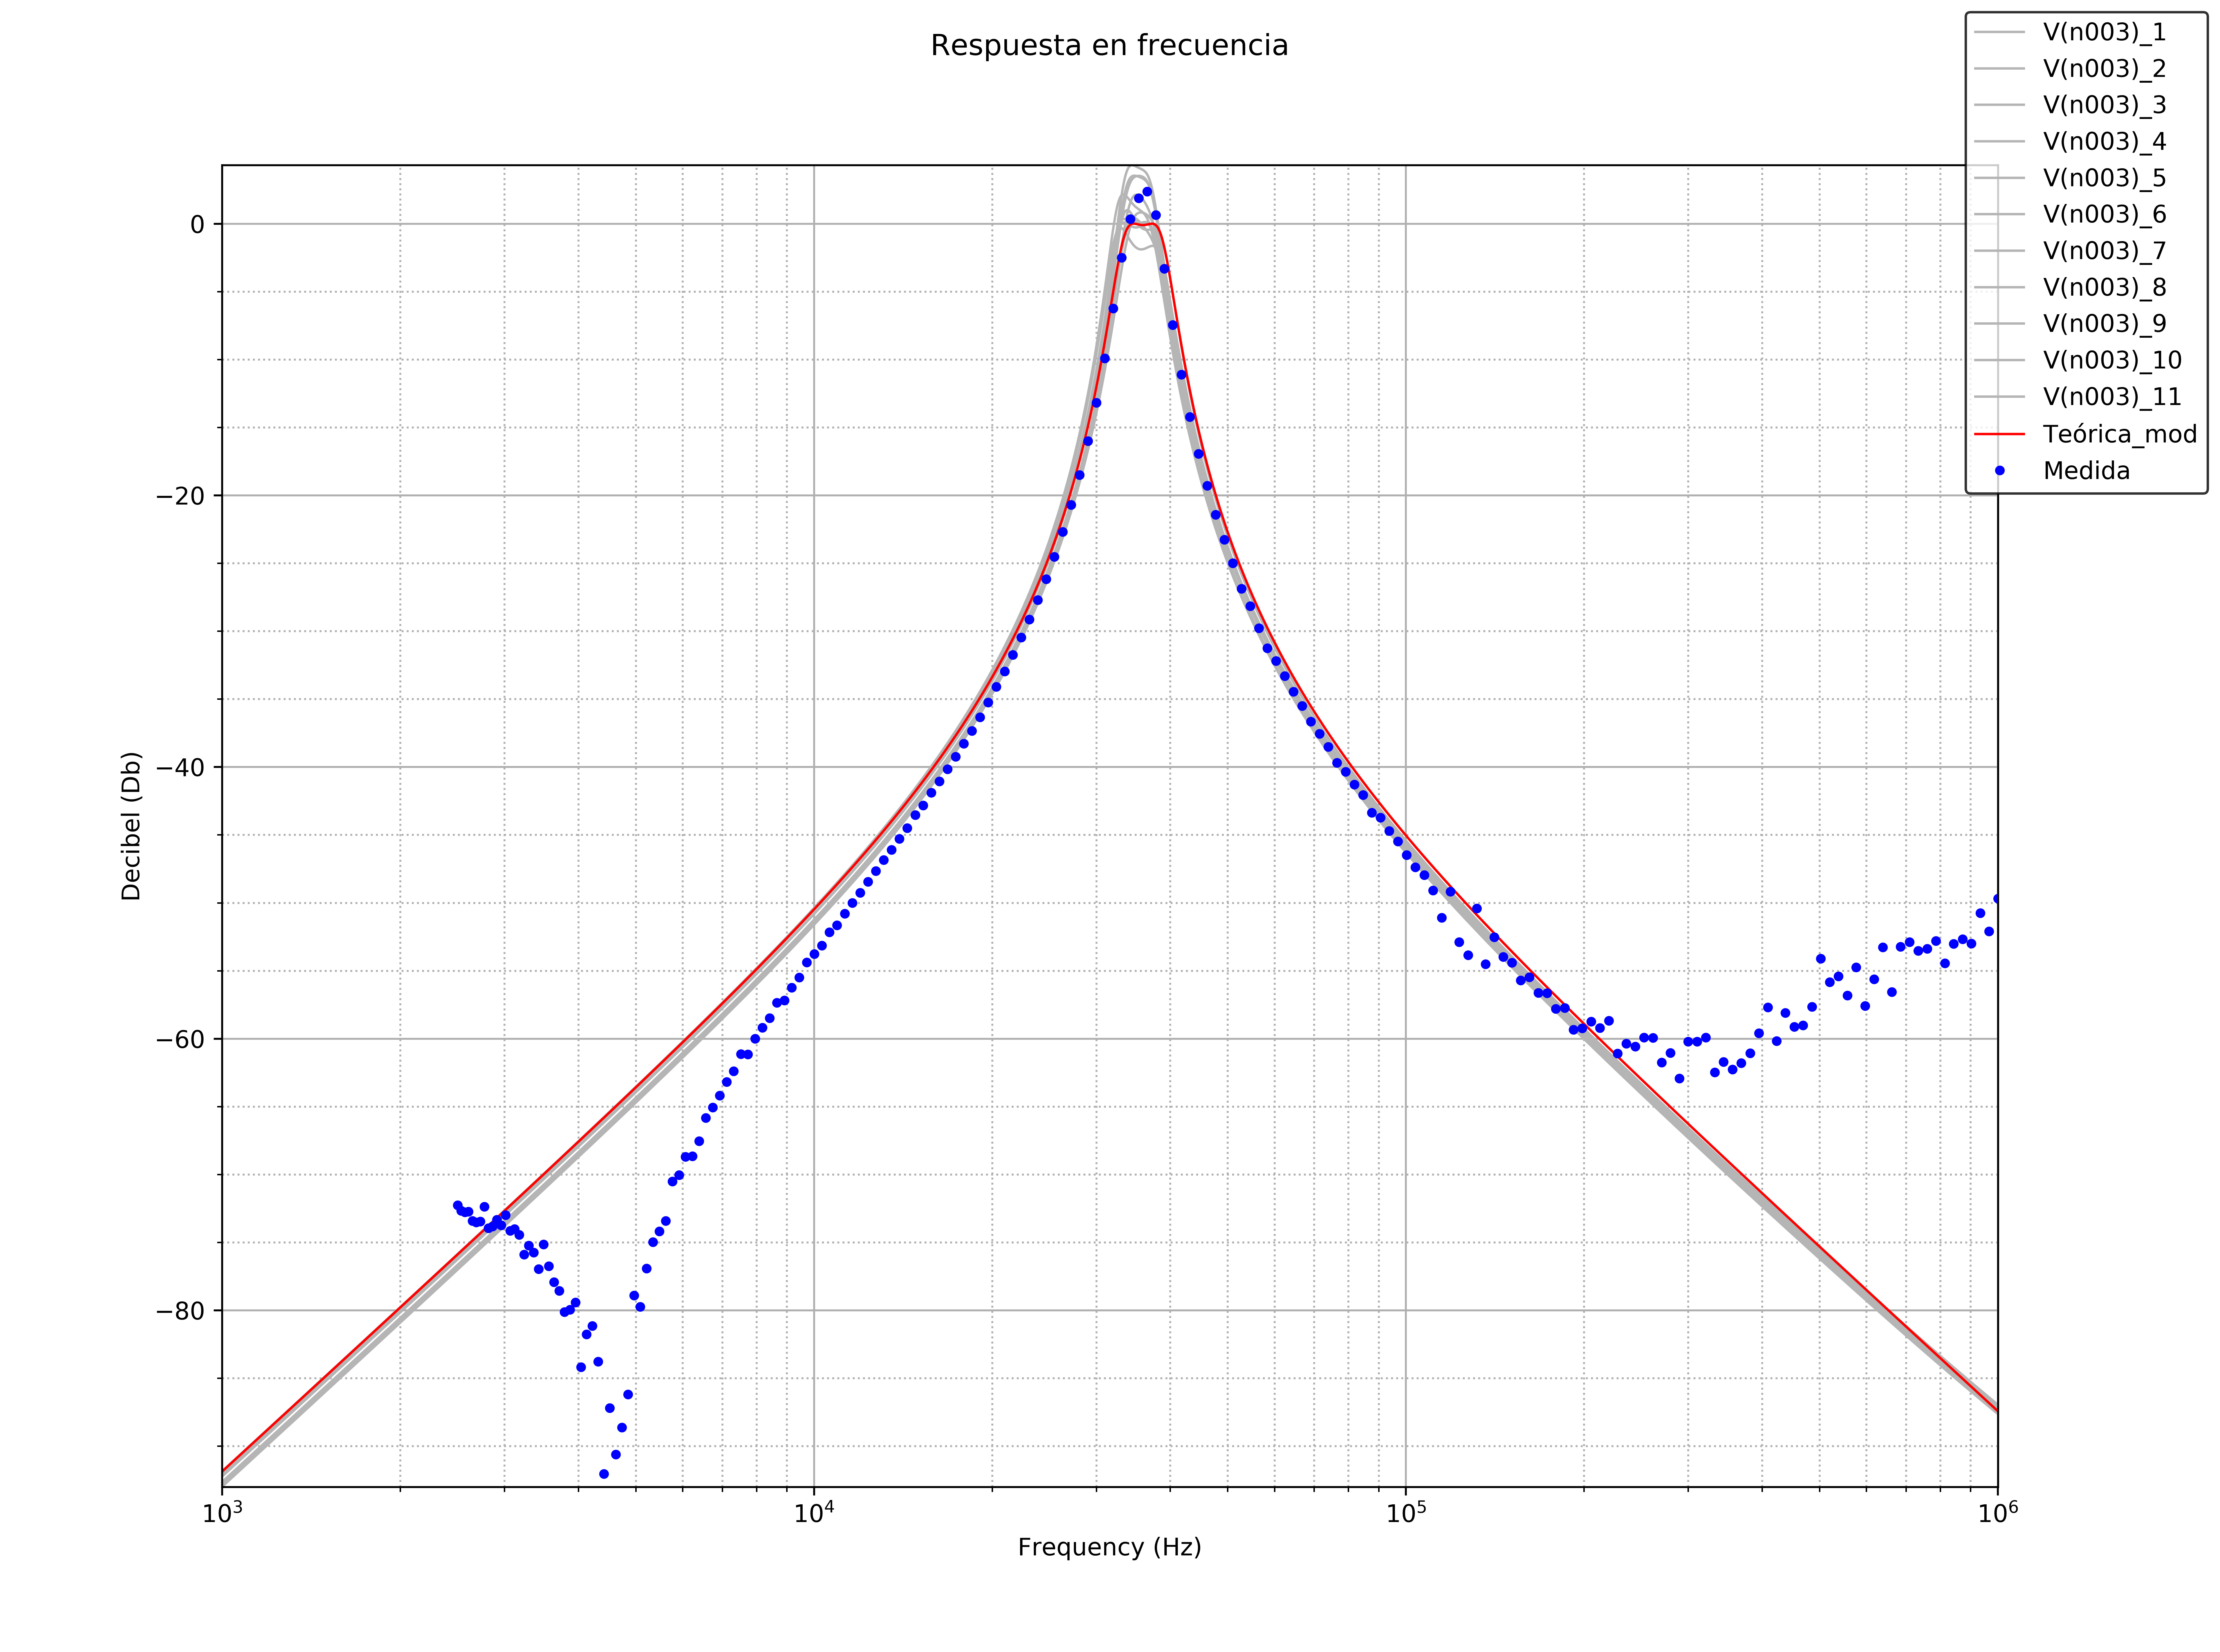
\includegraphics{../EJ2/Recursos/COMP_MOD} &
        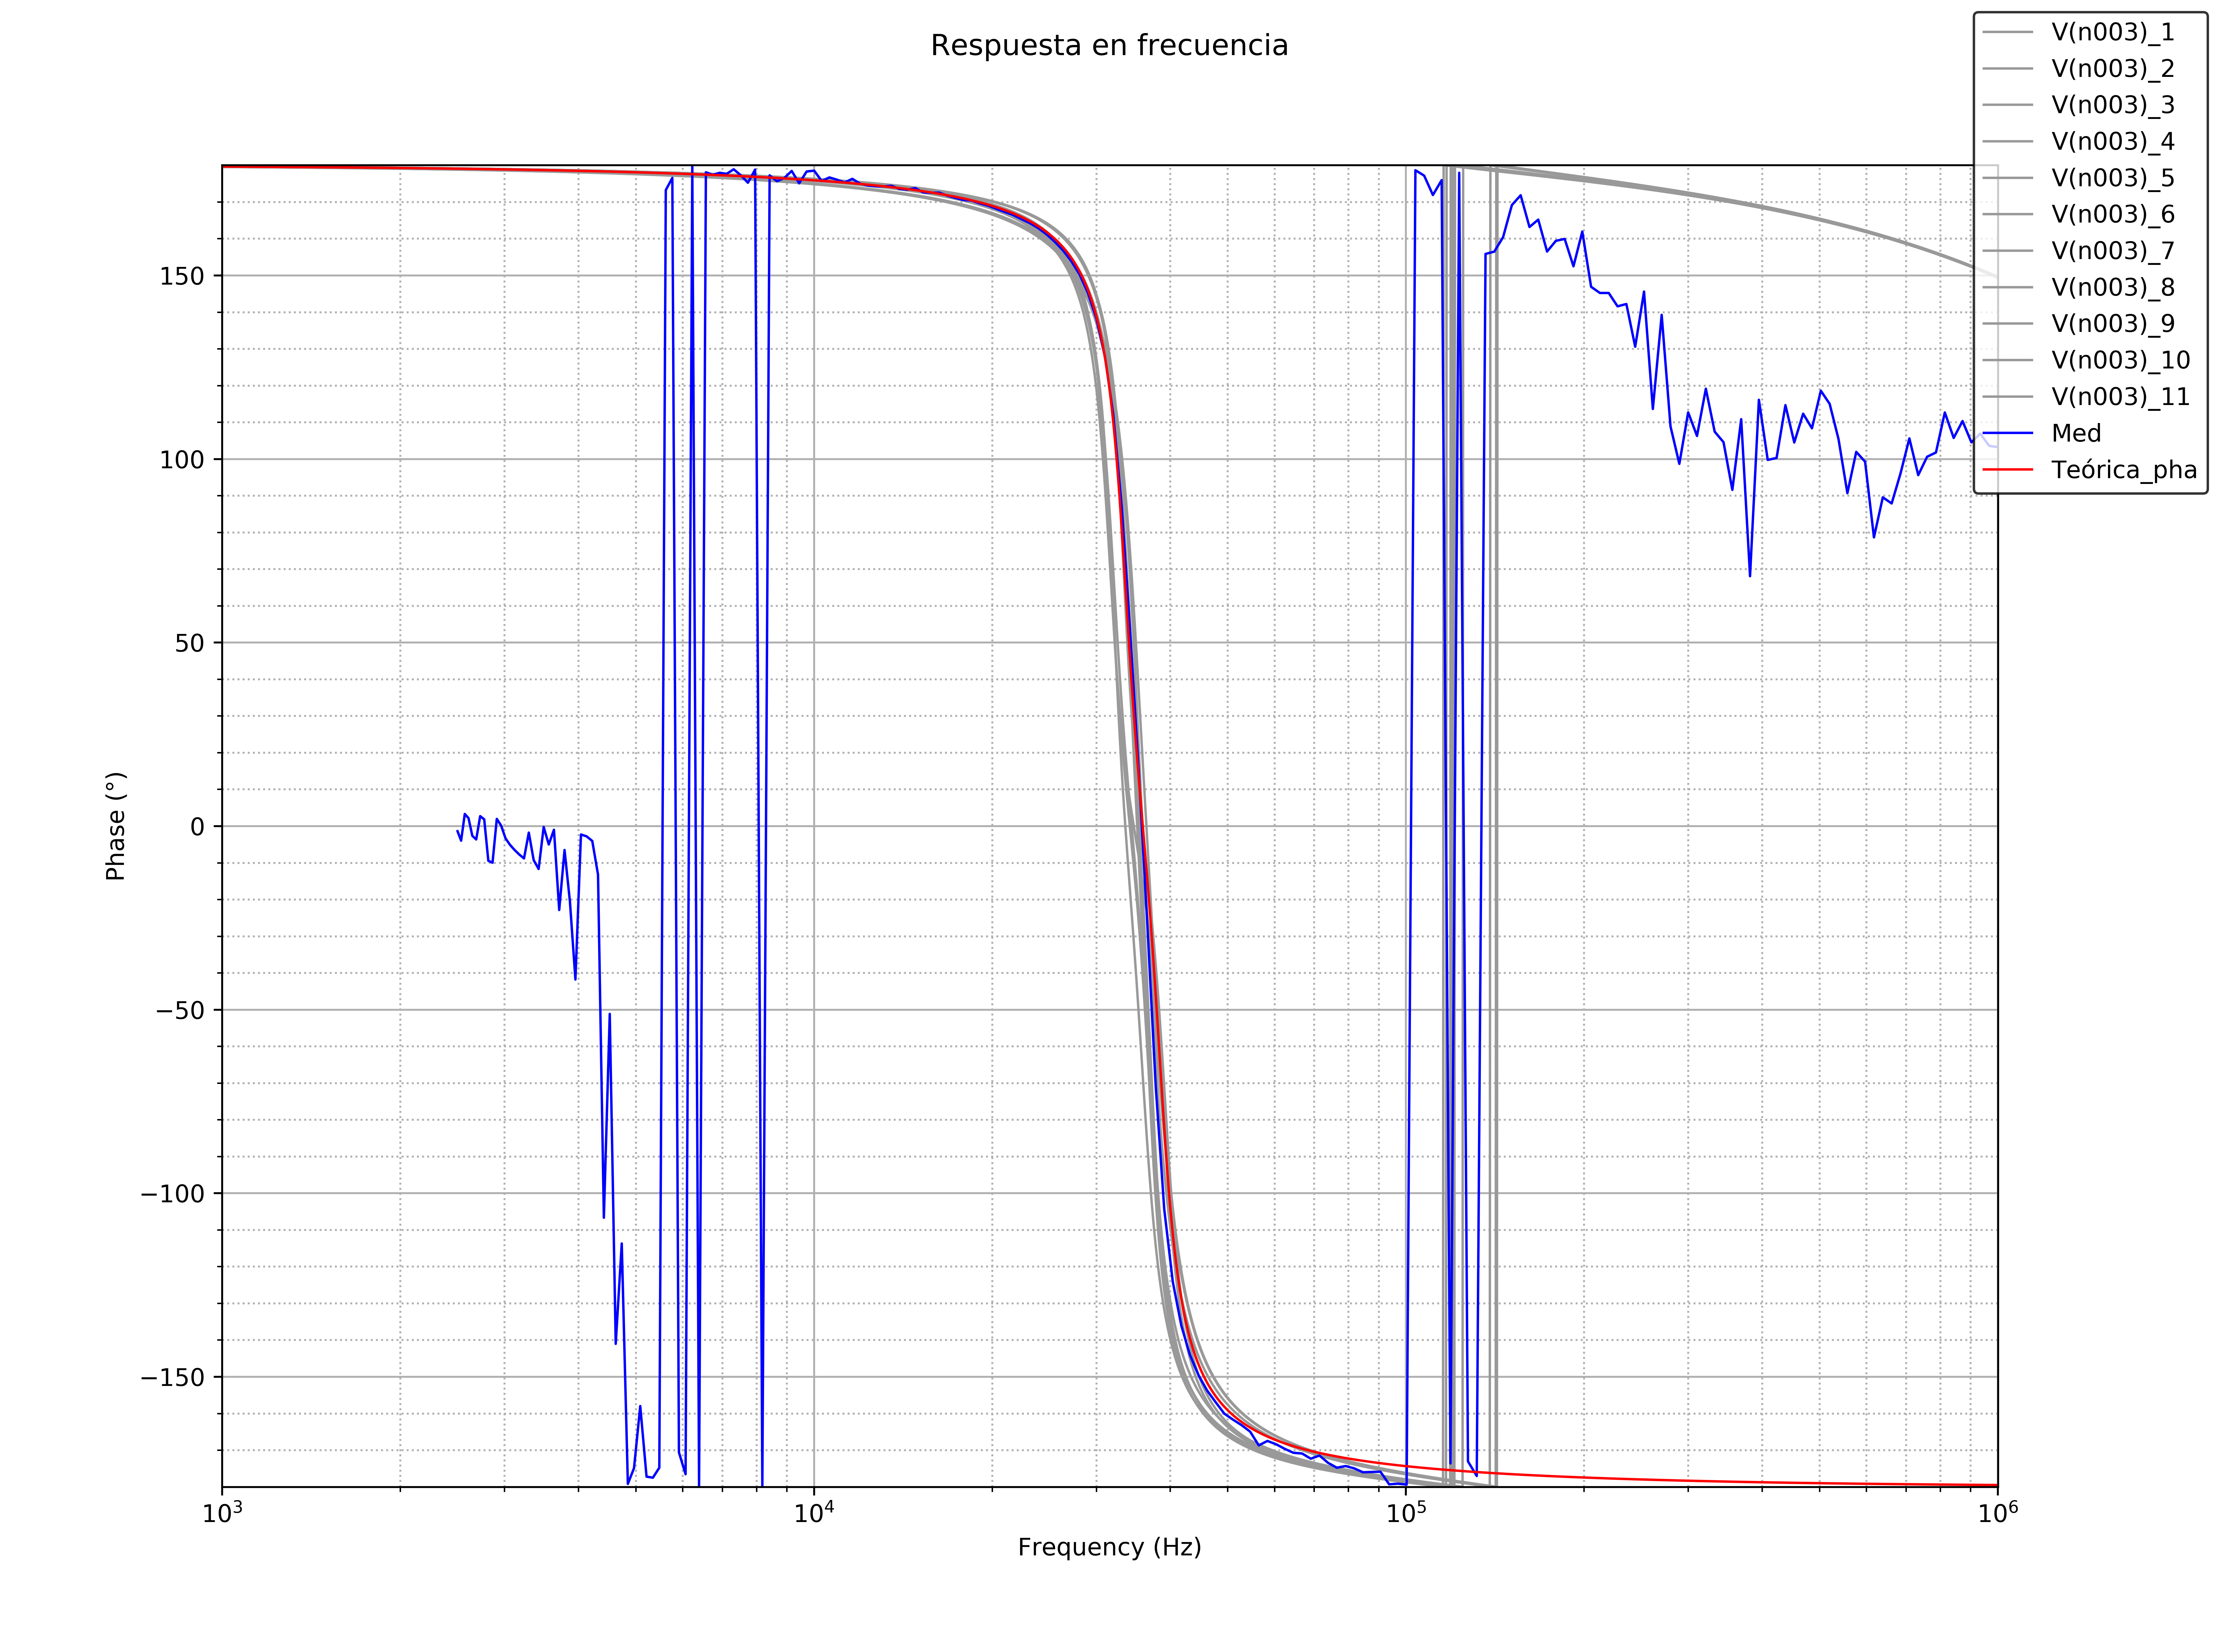
\includegraphics{../EJ2/Recursos/COMP_PHA} \\        
    \end{tabular}
    }
    \caption{Diagrams de m\'odulo y fase de la transferencia de todo el 
    filtro}
    \label{fig:COMP_BODE}
\end{figure}
\begin{figure}[H]
    \centering
    \resizebox{0.8\textwidth}{!}{%        
        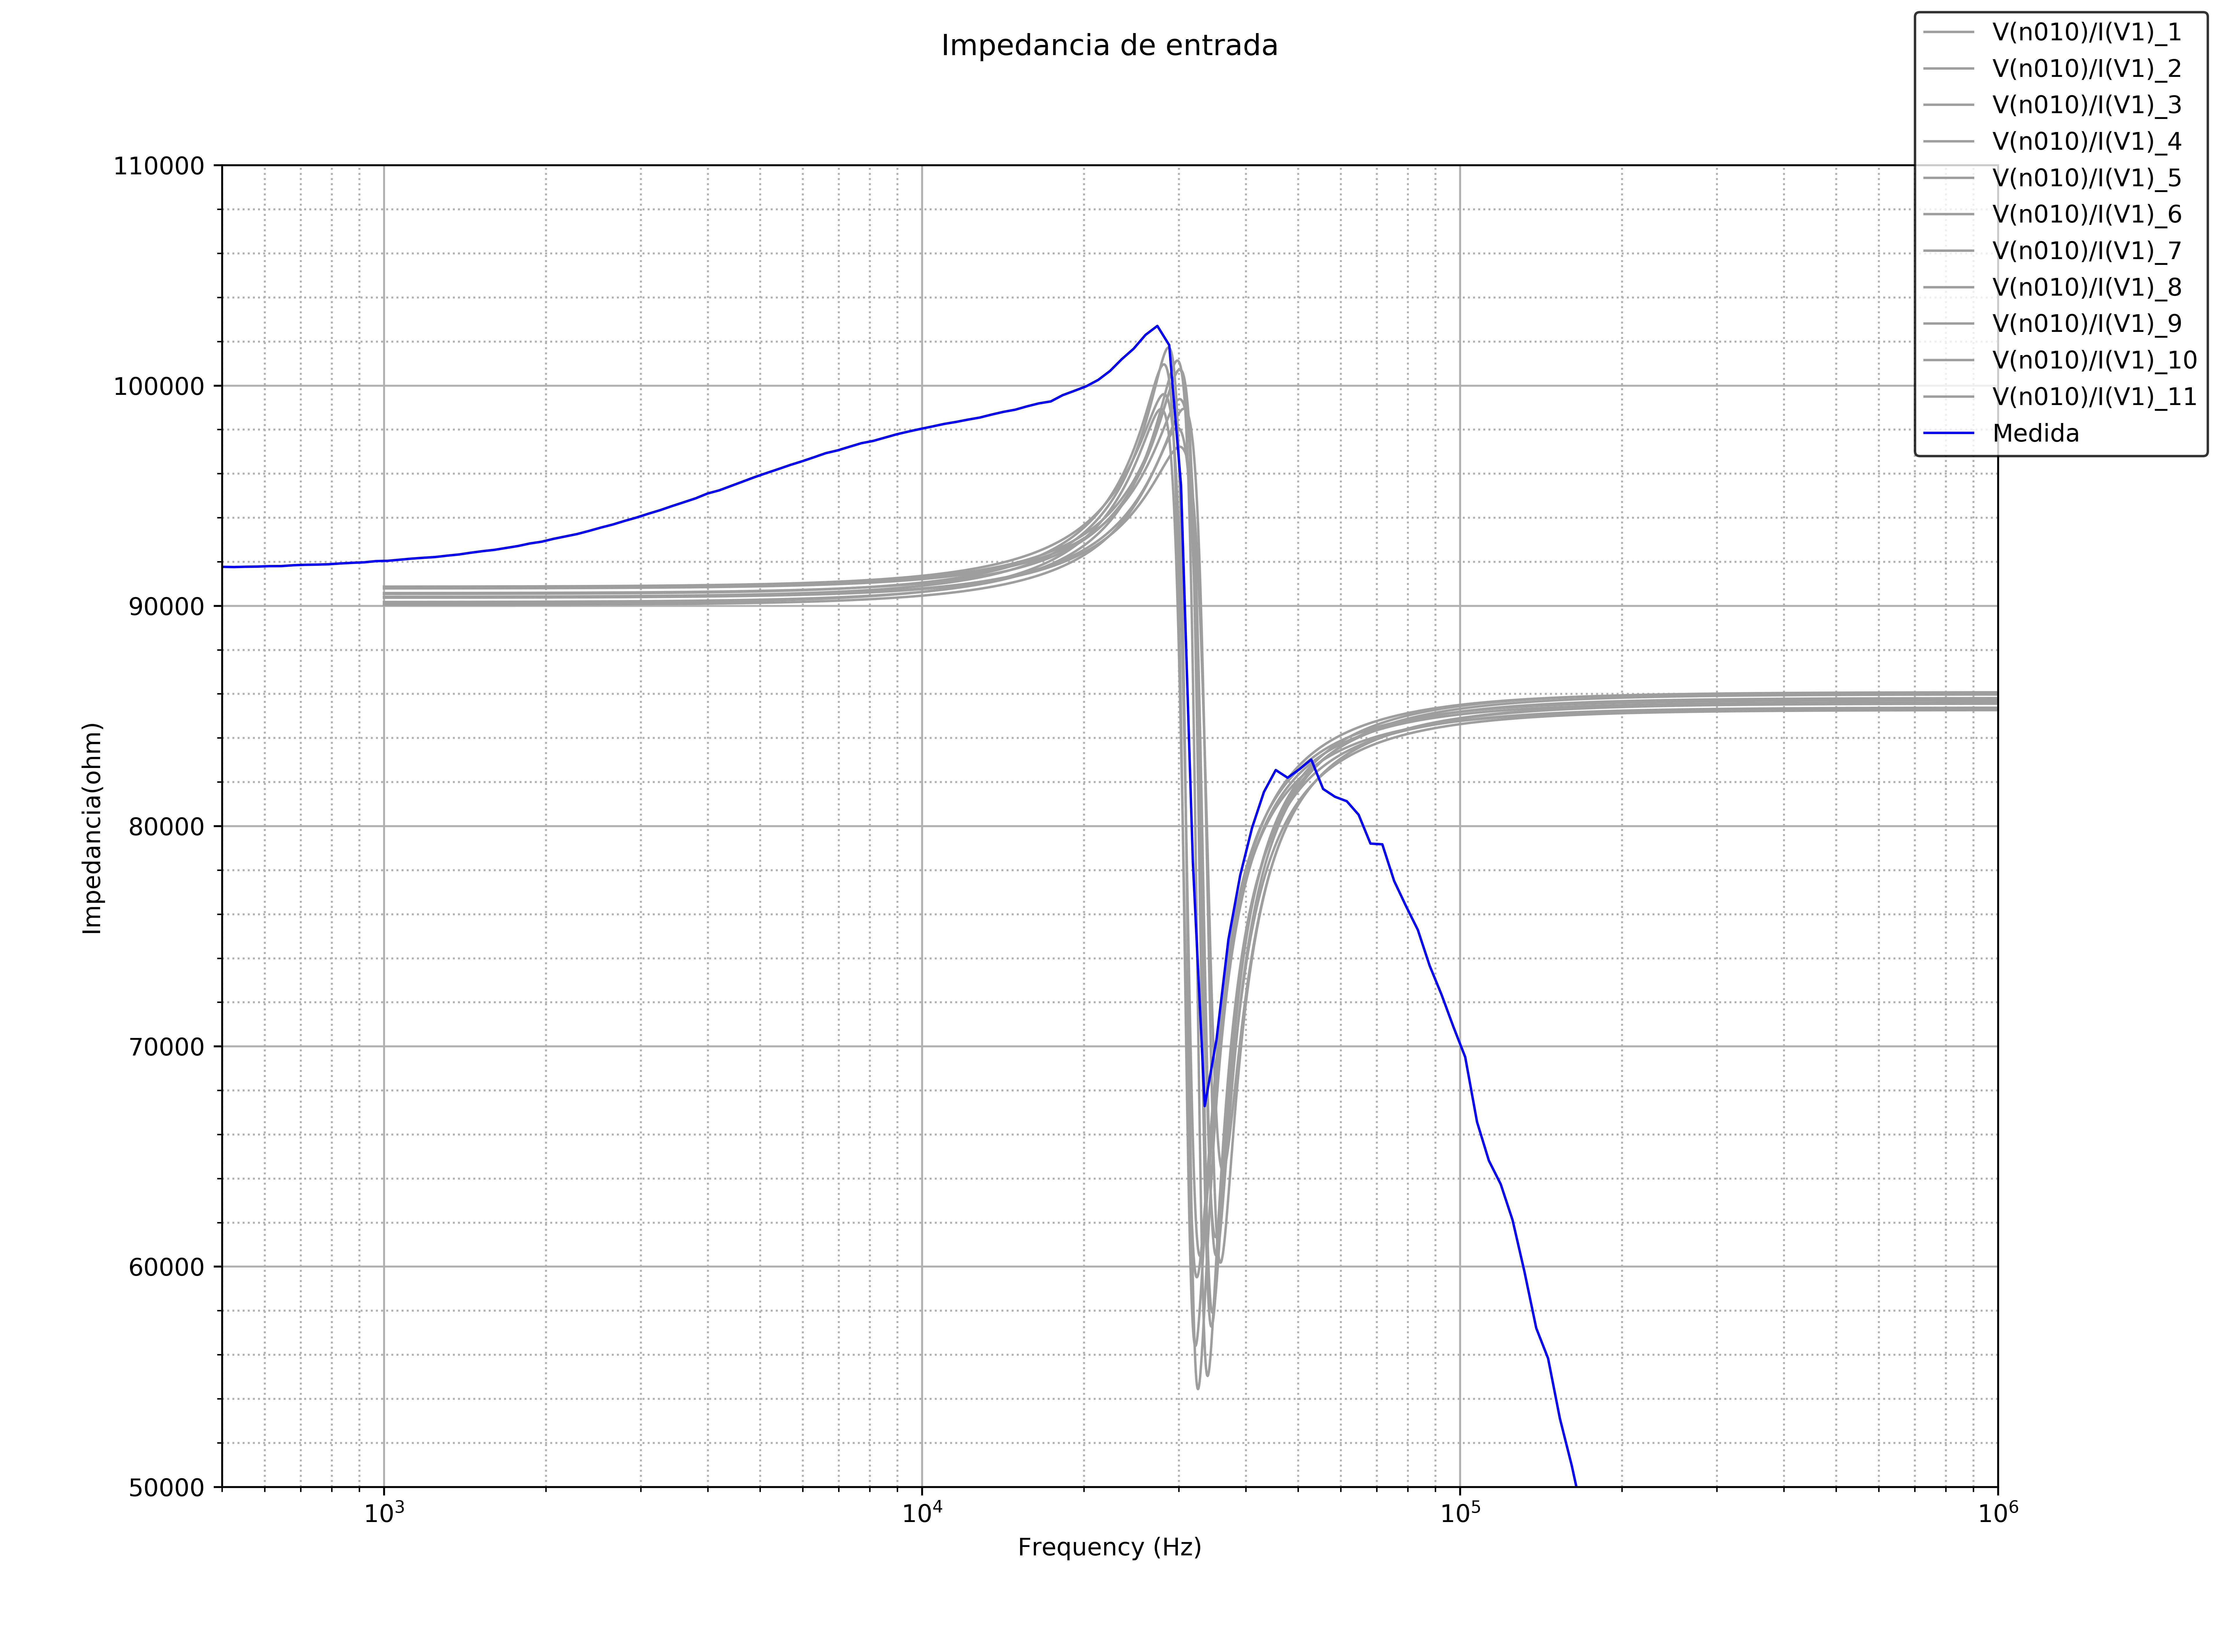
\includegraphics{../EJ2/Recursos/COMP_ZIN}       
    }
    \caption{Comparaci\'on de impedancia de entrada}
    \label{fig:ZIN}
\end{figure}
En todos los casos puede observarse que se corresponden correctamente los valores medidos con los calculados y los te\'oricos exepto por 2 cuestiones principales. La primera, como se menciona anteriormente, se obseva e algunas regiones de la banda pasante una gananacia de hasta 2dB, lo que no es deseable. Pero dado el nivel de variaciones debido a la tolerancia de los componentes y dado de que se encuentra dentro de los resultados esperados, se decide mantener.

El segundo aspecto, y en donde se encuentra la mayor variaci\'on respecto de las simulaciones, es la impedancia de entrada. Se puede observar en el gr\'afico que a partir de aproximadamente 150KHz la impedancia de entrada medida comienza a bajar por debajo de los $50K\Omega$ requeridos en la plantilla. Se atribuye esta diferencia al comportamiento en frecuencia de los componentes utilizados. La forma m\'as efectiva y r\'apida de solucionar este defecto es conectando un buffer a la entrada del filtro, lo que subir\'ia la impedancia de entrada y la volver\'ia idealmente independiente de lo que hay conectado a la salida.


\subsubsection{Rango din\'amico}
Se calcula el rango din\'amico utlizando la mayor ganancia medida, que es de $G=2.37dB = 1.313 veces$. La tensi\'on m\'axima a la salida ser\'a 13V teniendo en cuenta que la alimentaci\'on $\pm 15V$. Por lo tanto, para hallar la m\'axima tension a la entrada basta con realizar el c\'alculo mostrado a continuaci\'on
\begin{equation}
    V_i^{MAX} = \frac{V_o^{MAX}}{1.313} = 9.9V
\end{equation}
\newline\noindent
Luego, suponiendo que la  tensi\'on m\'inima distinguible es el piso de ruido, ya que por debajo de este nivel de tensi\'on no es posible distinguir entre la se\~nal y el ruido y asumiendo que este se encuentra en 10mV, se considera$V_o^{MIN}=10mV$.
\begin{equation}
    V_i^{MIN} = 10mV
\end{equation}
\newline\noindent
Utilizando estos valores se porcede a calcular el rango din\'amico (RD) como se muestra a continuaci\'on:
\begin{equation}
    RD = 20log(\frac{V_i^{MAX}}{V_i^{MIN}})= 59.91dB
\end{equation}

\subsection{Conclusiones}
Se puede observar que las celdas Rauch son \'utiles para implementar filtros pasabanda con elevados valores de factor de calidad. A pesar de esto, las sensibilidades tienen valores mas altos que el resto de las celdas, por lo que ajustar los valores de resistencias y capacitores puede ser dif\'icil. Adem\'as, esta celda en particular, dise\~nada para poder trabajar con altos valores de factor de calidad, funciona utilizando una realimentaci\'on positiva, por lo que es de suma importancia regular con precisi\'on los parametros que la controlan para evitar oscilaciones.